%%%%%%%%%%%%%%%%%%%%%%%%%%%%%%%%%%%%%%%%%
% Stylish Article
% LaTeX Template
% Version 2.1 (1/10/15)
%
% This template has been downloaded from:
% http://www.LaTeXTemplates.com
%
% Original author:
% Mathias Legrand (legrand.mathias@gmail.com) 
% With extensive modifications by:
% Vel (vel@latextemplates.com)
%
% License:
% CC BY-NC-SA 3.0 (http://creativecommons.org/licenses/by-nc-sa/3.0/)
%
%%%%%%%%%%%%%%%%%%%%%%%%%%%%%%%%%%%%%%%%%

%----------------------------------------------------------------------------------------
%	PACKAGES AND OTHER DOCUMENT CONFIGURATIONS
%----------------------------------------------------------------------------------------

\documentclass[fleqn,10pt]{SelfArx} % Document font size and equations flushed left

\usepackage[italian]{babel} % Specify a different language here - english by default

\usepackage{float}
%----------------------------------------------------------------------------------------
%	COLUMNS
%----------------------------------------------------------------------------------------

\setlength{\columnsep}{0.55cm} % Distance between the two columns of text
\setlength{\fboxrule}{0.75pt} % Width of the border around the abstract

%----------------------------------------------------------------------------------------
%	COLORS
%----------------------------------------------------------------------------------------

\definecolor{color1}{RGB}{0,0,90} % Color of the article title and sections
\definecolor{color2}{RGB}{0,20,20} % Color of the boxes behind the abstract and headings

%----------------------------------------------------------------------------------------
%	HYPERLINKS
%----------------------------------------------------------------------------------------

\usepackage{hyperref} % Required for hyperlinks
\hypersetup{hidelinks,colorlinks,breaklinks=true,urlcolor=color2,citecolor=color1,linkcolor=color1,bookmarksopen=false,pdftitle={Title},pdfauthor={Author}}

%----------------------------------------------------------------------------------------
%	ARTICLE INFORMATION
%----------------------------------------------------------------------------------------

\JournalInfo{Progetto di \textit{Foundation of Probability and Statistics}, Università degli Studi di Milano Bicocca} % Journal information
\Archive{Anno Accademico 2019-20} % Additional notes (e.g. copyright, DOI, review/research article)

\PaperTitle{Spotify Dataset - Analisi delle tracce musicali e previsione della popolarità} % Article title

\Authors{Riccardo Cervero\textsuperscript{1}} % Authors
\affiliation{\textsuperscript{1}\textit{794126, Dipartimento di Informatica, Sistemistica e Comunicazione}} % Author affiliation

\Keywords{Inferenza - Regressione lineare} 
\newcommand{\keywordname}{Keywords} 

%----------------------------------------------------------------------------------------
%	ABSTRACT
%----------------------------------------------------------------------------------------

\Abstract{Durante l'ultimo ventennio, grazie allo sviluppo di applicazioni \textit{web} per l'ascolto sempre più efficienti, la fruizione di contenuti musicali ha mostrato un'importante e rapida evoluzione, permettendo all'utente di accedere a qualsiasi brano - o qualunque versione dello stesso - in brevissimo tempo e, nella maggior parte dei casi, gestire autonomamente un archivio di tracce e artisti preferiti. L'industria discografica ha saputo sfruttare tale progresso, non soltanto incrementando il volume di distribuzione e di campagne promozionali, ma anche approfondendo quantitativamente e qualitativamente le tendenze d'ascolto di un pubblico catalogato. Moderne piattaforme offrono, infatti, la possibilità di estrarre ed analizzare una vasta varietà di parametri acustici e non, cosicché il produttore possa dedurre quali sono le caratteristiche più ricercate dal pubblico in un determinato momento e aumentare così la popolarità delle proprie canzoni. È il caso, ad esempio, di \textit{Spotify}. Questo progetto, pertanto, ha come obiettivo l'analisi statistica delle caratteristiche qualitative e quantitative registrate da \textit{Spotify} in un \textit{database} di tracce disponibili all'interno del proprio servizio di \textit{streaming musicale}. Più precisamente, nella seconda e terza sezione verranno esaminate le variabili,  testata la loro reciproca connessione - di tipo lineare o non - e calcolate stime intervallari per le rispettive medie o proporzioni fra le modalità. Infine, nelle due successive sezioni, verranno esposti i risultati dei modelli di regressione lineare - sia semplice che multivariata - per la previsione della popolarità del brano e della positività emotiva da esso trasmessa.} 

%----------------------------------------------------------------------------------------

\begin{document}

\flushbottom % Makes all text pages the same height

\maketitle % Print the title and abstract box

\tableofcontents % Print the contents section

\thispagestyle{empty} % Removes page numbering from the first page

%----------------------------------------------------------------------------------------
%	ARTICLE CONTENTS
%----------------------------------------------------------------------------------------

\section{Caso di studio}
I dati esaminati nell'ambito di questo progetto provengono dal database di \textit{Kaggle} "Spotify Dataset"\footnote{Il link da cui è possibile scaricare il database "Spotify Dataset" è \href{https://www.kaggle.com/yamaerenay/spotify-dataset-19212020-160k-tracks}{\texttt{/kaggle/spotify-dataset-160k-tracks}}.}, che raccoglie un totale di 19 caratteristiche acustiche e qualitative relative a 169909 tracce, rese disponibili sulla piattaforma \textit{Spotify for Developers}.\footnote{La documentazione della piattaforma \textit{Spotify for Developers} è disponibile al link \href{https://developer.spotify.com}{\texttt{developer.spotify.com}}.}\\
Le variabili oggetto di studio\footnote{La descrizione ufficiale delle variabili è disponibile ai link \href{https://developer.spotify.com/documentation/web-api/reference/tracks/get-audio-features/}{\texttt{developer.spotify/audio-features}} e \href{https://developer.spotify.com/documentation/web-api/reference/tracks/get-track/}{\texttt{developer.spotify/get-track}}.} corrispondono alle seguenti grandezze:
\begin{itemize}
    \item \textit{Acousticness} - o "acusticità" , è misura numerica - fra 0 e 1 - della confidenza con cui è possibile definire "acustica" una traccia: se 1, indica massima certezza nell'affermare che il brano sia stato prodotto senza strumenti elettronici
    \item \textit{Danceability} è il grado di ballabilità calcolato fra 0 e 1, come combinazione di vari elementi musicali, fra cui la stabilità del ritmo e il tempo
    \item \textit{Duration} è la durata del brano in millisecondi
    \item \textit{Energy} rappresenta la percentuale di intensità della traccia, sulla base di elementi percettivi quali sonorità e timbro
    \item \textit{Explicit} è variabile binaria che rileva la presenza o meno di contenuto esplicito
    \item \textit{Instrumentalness} misura, fra 0 e 1, l'assenza di contenuto vocale: più il valore si avvicina a 1, maggiore è la confidenza con cui si definisce "strumentale" la traccia
    \item \textit{Key} registra la stima della chiave complessiva della traccia, codificata in un valore numerico compreso fra 0 (Do) e 11 (Si)
    \item \textit{Liveness} rileva la presenza di un pubblico udibile nella registrazione, definendone la probabilità: se superiore a 0,8, fornisce una forte evidenza che la traccia sia stata registrata dal vivo
    \item \textit{Loudness} è il volume complessivo in decibel, fra -60 e circa 4
    \item \textit{Mode} è la variabile binaria circa la tonalità del brano: 1 se maggiore, 0 se minore
    \item \textit{Speechiness} indica la presenza di parlato: maggiore la somiglianza tra la traccia e un discorso - come nel caso del genere \textit{rap} -, maggiore la vicinanza del valore a 1
    \item \textit{Tempo} è il ritmo misurato in battiti al minuto (bpm)
    \item \textit{Valence} definisce il grado di positività emotiva trasmessa dal brano, tra 0 e 1
    \item \textit{Year} è l'anno di uscita del brano, dal 1921 al 2020
    \item \textit{Popularity} è una variabile intera compresa fra 0 e 100, che esprime il grado di popolarità del brano, calcolato a partire dal numero totale di riproduzioni su \textit{Spotify} e da quanto sono recenti tali ascolti: in generale, tracce riprodotte molto frequente durante l'anno corrente avranno un valore di popolarità molto elevato
\end{itemize}
Tali colonne verranno presentate singolarmente nei diversi paragrafi delle Sezioni \ref{cqual} e \ref{cquant}. In particolare, la popolarità verrà considerata come principale variabile \textit{target} nell'ambito della definizione di modelli di regressione.\\
\subsection{Pre-processing}
Il dataset originale non presentava alcun valore mancante, e le uniche operazioni di \textit{pre-processing} hanno implicato il raggruppamento delle modalità dell'anno di pubblicazione in classi di decennio (Sezione \ref{year}) e la rimozione delle variabili poco interessanti per l'obiettivo di analisi statistica: l'identificatore primario della traccia, il titolo, la lista di artisti accreditati e la data di pubblicazione. In particolare, la data di pubblicazione \textit{Release\_date} si manifestava in formato YYYY-MM-DD soltanto nel 70\% dei casi, mentre la restante parte riportava soltanto l'anno, così come la colonna \textit{Year}. Non potendo risalire al mese e al giorno, si è preferito eliminare \textit{Release\_date}.
%------------------------------------------------
\section{Analisi dei caratteri qualitativi}\label{cqual}
\subsection*{Variabile \textit{Year}}\label{year}
Le osservazioni del database "Spotify Dataset" sono distribuite con una certa coerenza fra i singoli anni - dal 1921 al 2020: le frequenze relative delle modalità di \textit{Year} sono identiche o comunque molto simili a 0.012 - che corrisponde alla frequenza relativa massima - in 73 anni su 100. Osservazioni meno numerose sono comprensibilmente relative agni anni precedenti al 1947. Perciò, la distribuzione di questa variabile qualitativa ordinale, oltre ad essere multimodale, può anche essere definita estremamente eterogenea: infatti, la mutabilità del fenomeno, misurata dall'indice normalizzato di Gini, mostra un valore di 0.999.\\
Poichè è noto che le tendenze musicali possono essere meglio definite nell'arco di decadi, piuttosto che di singole stagioni, si è deciso di aggregare le osservazioni per decenni. Le rispettive frequenze delle decadi sono intuibili in Figura \ref{fig:fig1}. 
\begin{figure}[H]
    \centering
    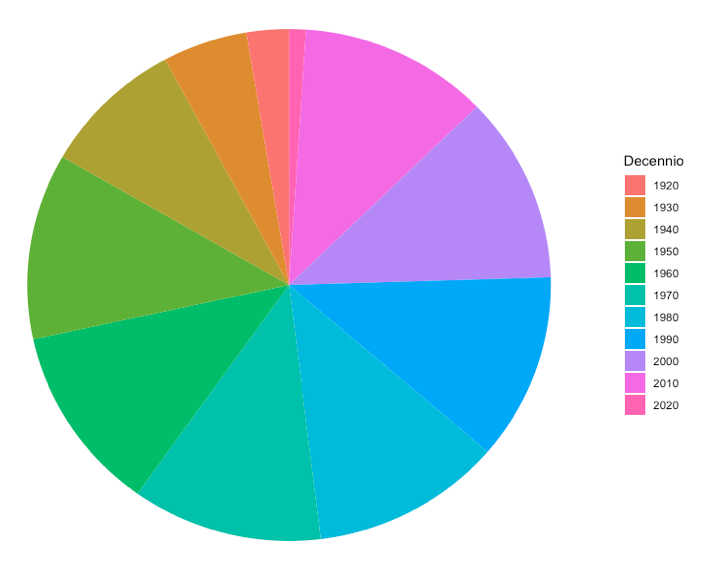
\includegraphics[width=0.7 \linewidth]{fig1.png}
    \caption{Aerogramma per la visualizzazione delle frequenze relative dei decenni.}
    \label{fig:fig1}
\end{figure}
Si è poi proceduto a verificare l'esistenza di una connessione fra questa nuova variabile e il grado di popolarità dei brani, eseguendo un test Chi-quadrato, cui ipotesi nulla
\begin{equation}
  H_0:\chi^2=0  
\end{equation}
coincide con l'indipendenza statistica fra i due fenomeni. L'indice di associazione $\chi^2$ è dunque calcolato con $(k_1-1)(k_2-1)=990$ gradi di libertà, con $k_1=11$ e $k_2=100$ i rispettivi conteggi delle modalità. Fissato un livello di significatività $\alpha=0.05$, è stato ottenuto un valore \textit{pvalue} considerevolmente inferiore ad $\alpha$\footnote{Il \textit{pvalue} in questione è inferiore alla soglia $2.2\bullet10^{-16}$.}, portando a rifiutare, con confidenza al 95\%, l'ipotesi nulla di indipendenza fra il decennio di uscita della traccia e il proprio grado di popolarità. Ciò significa che le distribuzioni condizionate della popolarità variano in base alla decade considerata, come visibile in Figura \ref{fig:fig2}. 
\begin{figure}[H]
    \centering
    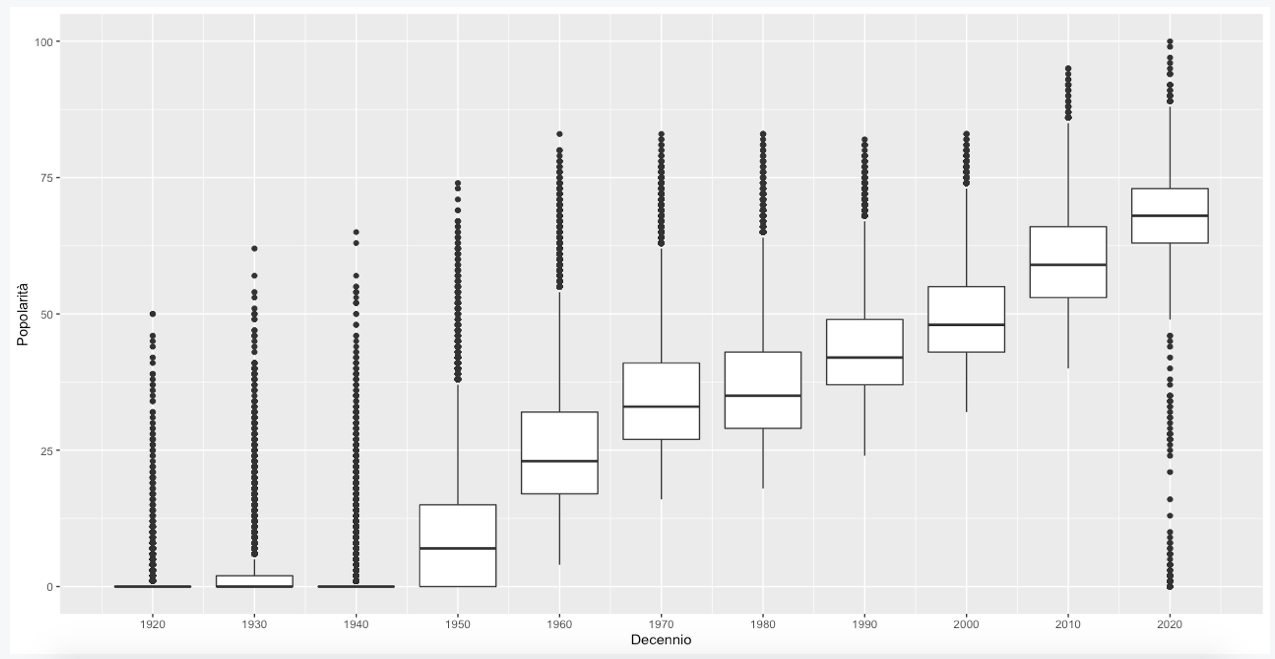
\includegraphics[width=1 \linewidth]{fig2.png}
    \caption{\textit{BoxPlot} condizionati per la visualizzazione delle distribuzioni condizionate di popolarità in base al decennio esaminato.}
    \label{fig:fig2}
\end{figure}
La natura di questa dipendenza statistica viene approfondita mediante test ANOVA, basato sull'ipotesi nulla di uguaglianza di tutte le popolarità medie, ovvero sull'ipotesi che le osservazioni di popolarità relative a ciascun decennio provengano da popolazioni che seguono una distribuzione normale con varianza e media pari. Si punta pertanto a verificare l'ipotesi alternativa, cioè che la media di almeno un gruppo differisca dalle altre, dimostrando che il fattore condizionante della decade ha un'influenza sulla popolarità. La statistica test è associata a 10 gradi di libertà e, fissato un livello di significatività $\alpha=0.05$, è stato ottenuto un valore \textit{pvalue} ancora una volta nettamente inferiore ad $\alpha$, causando il rifiuto dell'ipotesi nulla di uguaglianza delle popolarità medie per decennio e confermando, con una confidenza al 95\%, la presenza di una forte relazione fra queste due variabili. Osservando la Figura, è possibile riscontrare, almeno visivamente, una tendenza comprensibile: la preferenza degli utenti a livello aggregato appare quasi perfettamente ordinata per "novità" del brano.

\subsection*{Variabile \textit{Explicit}}
Un fenomeno, al contrario, distribuito in maniera poco equilibrata è la presenza di contenuto esplicito nel testo: la frequenza percentuale delle tracce non esplicite è pari al 91.51\% (Figura \ref{fig:fig3}) e il suo indice di Gini normalizzato conferma la bassa mutabilità: $\sim$0.311. 
\begin{figure}[H]
    \centering
    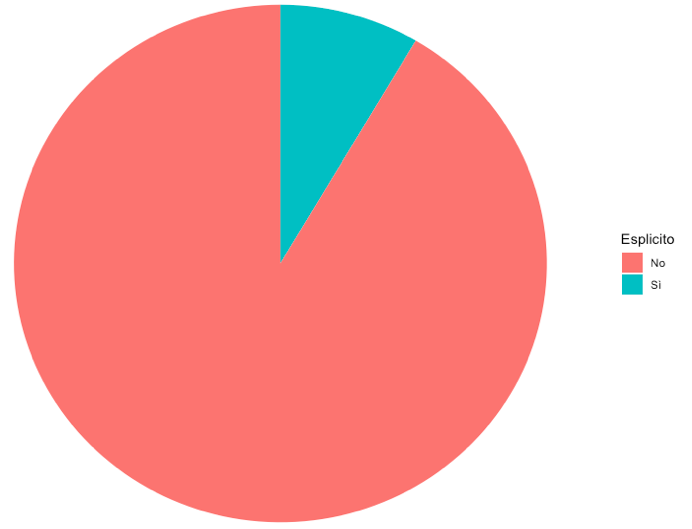
\includegraphics[width=0.7 \linewidth]{fig3.png}
    \caption{Aerogramma per la visualizzazione delle rispettive frequenze relative di contenuto esplicito e non esplicito.}
    \label{fig:fig3}
\end{figure}
Nonostante l'elevata numerosità del campione studiato, rimane più utile e affidabile la pratica di stima intervallare del parametro di proporzione $p$, che deriva dallo studio della distribuzione campionaria della frequenza relativa di una determinata classe nella popolazione. L'intervallo di confidenza ottenuto, avrà pertanto i seguenti estremi:
\begin{equation}
    (p-z_{\frac{\alpha}{2}}\sqrt{\frac{p(1-p)}{n}};p+z_{\frac{\alpha}{2}}\sqrt{\frac{p(1-p)}{n}})
\end{equation}
In questo caso, fissato un livello di significatività $\alpha=0.05$, i rispettivi intervalli di confidenza delle modalità "esplicito" e "non esplicito" - con estremi approssimati al terzo decimale - sono:
\begin{equation}
    (0.084, 0.086)\\(0.914, 0.916)
\end{equation}
Anche in questo caso, viene verificata l'esistenza di una connessione fra il grado di popolarità e la presenza di contenuto esplicito: ad un livello di confidenza del 95\% e con 99 gradi di libertà, l'ipotesi di indipendenza fra le due variabili viene rifiutata poiché il \textit{pvalue} è calcolato nettamente inferiore alla soglia di significatività.\\
Inoltre, eseguendo un test ANOVA sull'uguaglianza delle due popolarità medie in corrispondenza di contenuto esplicito e non esplicito, si ottiene un \textit{pvalue} molto basso, rifiutando nuovamente l'ipotesi nulla con un livello di confidenza al 95\%.
\begin{figure}[H]
    \centering
    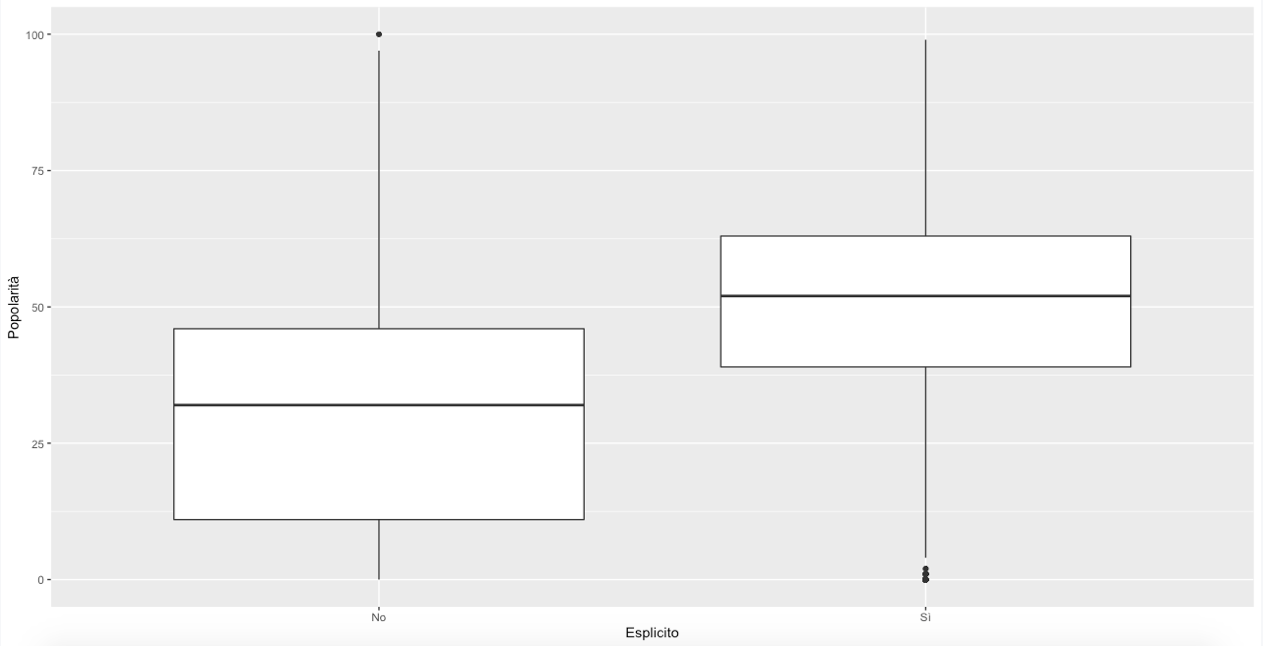
\includegraphics[width=1 \linewidth]{fig4.png}
    \caption{\textit{BoxPlot} condizionati per la visualizzazione delle distribuzioni condizionate di popolarità in base alla presenza o meno di contenuto esplicito.}
    \label{fig:fig4}
\end{figure}

\subsection*{Variabile \textit{Mode}}
La distribuzione delle due tonalità si presenta sbilanciata: la frequenza percentuale della modalità "maggiore" è circa il 70.9\%, contro il 29.1\% della "minore" (Figura \ref{fig:fig5}).
\begin{figure}[H]
    \centering
    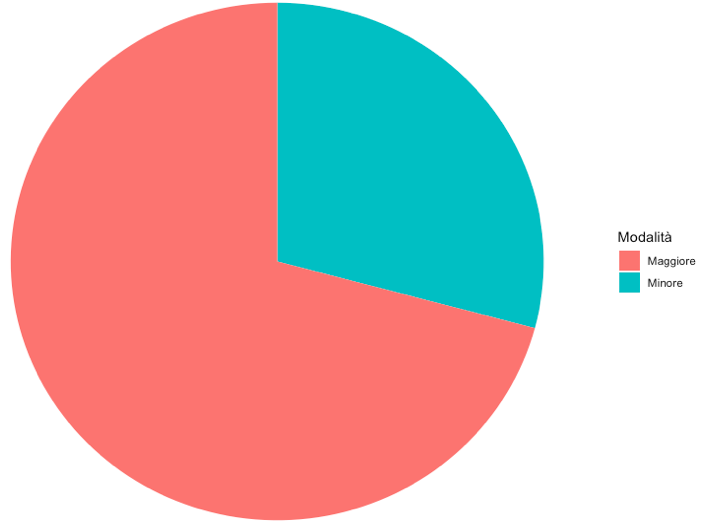
\includegraphics[width=0.7 \linewidth]{fig5.png}
    \caption{Aerogramma per la visualizzazione delle frequenze relative delle due tonalità.}
    \label{fig:fig5}
\end{figure}
L'indice di Gini normalizzato viene calcolato pari a 0.83.\\
Si è proceduto dunque ad estrarre un'informazione più accurata e affidabile tramite stima intervallare delle proporzioni di tracce in tonalità minore e maggiore nella popolazione: ad un livello di confidenza del 95\%, le rispettive probabilità sono contenute nei seguenti intervalli di confidenza - con estremi approssimati al terzo decimale:
\begin{equation}
    (0.289, 0.294)\\(0.706, 0.711)
\end{equation}
Viene rifiutata, ad un livello di confidenza del 95\%, l'ipotesi che l'indice di connessione $\chi^2$ per l'individuazione di una dipendenza statistica fra la tonalità del brano e la sua popolarità, calcolato con 99 gradi di libertà, sia nullo: il \textit{pvalue} ha un valore estremamente basso. Per lo stesso motivo, si rifiuta, tramite test ANOVA con $\alpha=0.05$, l'uguaglianza delle popolarità medie delle tracce condizionate alle due diverse tonalità.
\begin{figure}[H]
    \centering
    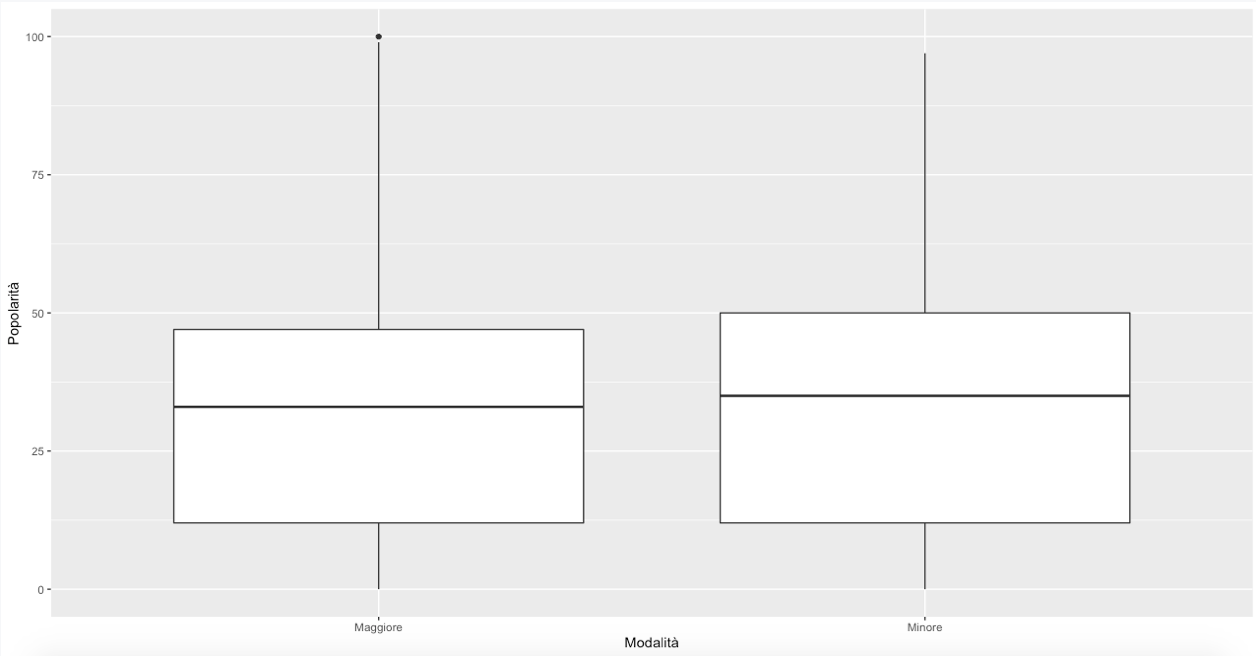
\includegraphics[width=1 \linewidth]{fig6.png}
    \caption{\textit{BoxPlot} condizionati per la visualizzazione delle distribuzioni condizionate di popolarità in base alla tonalità.}
    \label{fig:fig6}
\end{figure}

\subsection*{Variabile \textit{Key}}
L'ultimo carattere qualitativo, riferito alla chiave globale della traccia, mostra un'elevatissima eterogeneità: l'indice normalizzato di Gini è infatti pari a 0.991. È possibile, fra le 11 modalità, individuarne la moda: la chiave di "Do", con una frequenza percentuale del 12.65\%. Tuttavia, per poter affermare con più affidabilità che la chiave più frequente fra i brani musicali sia effettivamente "Do", è necessario confrontare le rispettive stime intervallari delle frequenze relative di tutte le modalità di \textit{Key}. Il risultato di ogni stima è riassunto in Figura \ref{fig:fig8}. Poiché gli estremi superiori degli intervalli di confidenza delle altre chiavi sono sempre minori rispetto al limite inferiore dell'intervallo di confidenza di "Do", è possibile affermare con un livello di confidenza del 95\% che essa sia, in effetti, la chiave più usata per comporre una traccia. Allo stesso modo, "Re diesis" può essere considerata come la chiave meno utilizzata.
\begin{figure}[H]
    \centering
    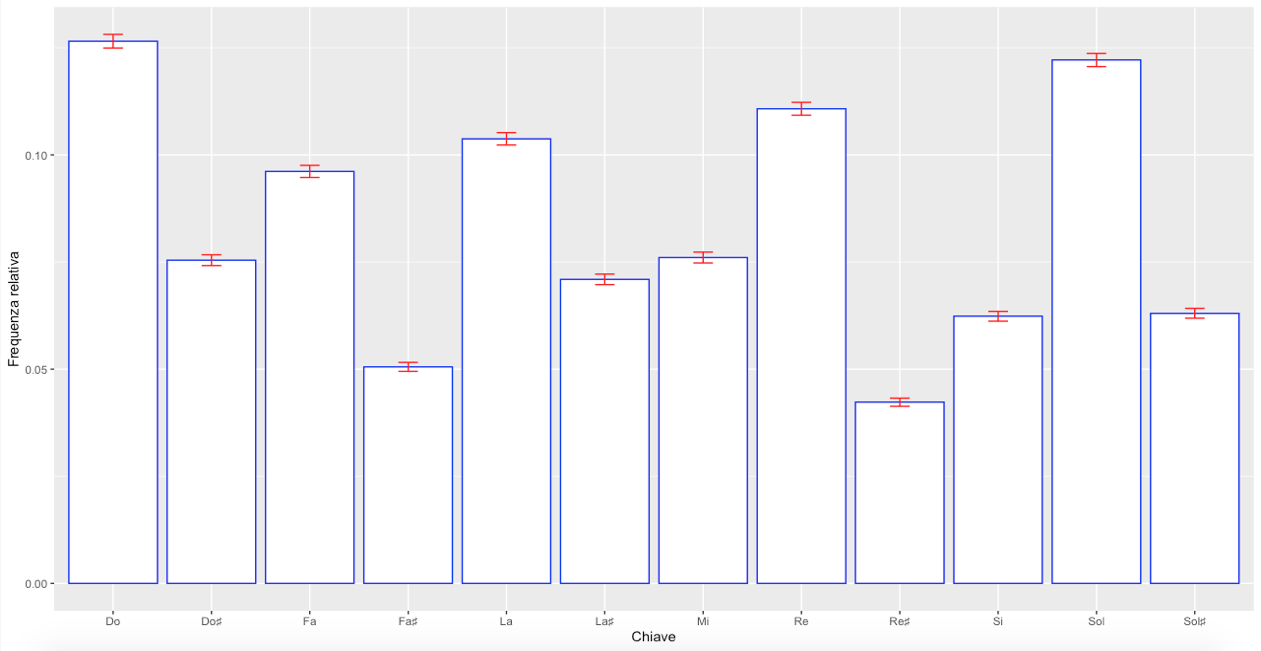
\includegraphics[width=1 \linewidth]{fig8.png}
    \caption{\textit{BarPlot} delle frequenze relative di ciascuna chiave nella popolazione. I segmenti rossi verticali indicano gli intervalli di confidenza calcolati con $(1-\alpha)=0.95$. Dall'osservazione del grafico, è possibile dedurre che "Do" sia la chiave più frequente.}
    \label{fig:fig8}
\end{figure}
Viene poi rifiutata, con un livello di significatività $\alpha=0.05$, l'ipotesi di indipendenza statistica fra la popolarità e la chiave. Infine, eseguendo un test ANOVA con livello di confidenza del 95\%, si rifiuta anche l'ipotesi di uguaglianza fra le popolarità medie condizionate alla chiave globale con cui è stata composta la traccia. Ciò significa che la scelta della chiave, così come la selezione di una determinata tonalità e l'introduzione di contenuto esplicito nel testo, ha un'influenza sul livello di popolarità che raggiungerà il brano.\\
In Figura \ref{fig:fig9}, è possibile osservare le distribuzioni della popolarità condizionata alla chiave.
\begin{figure}[H]
    \centering
    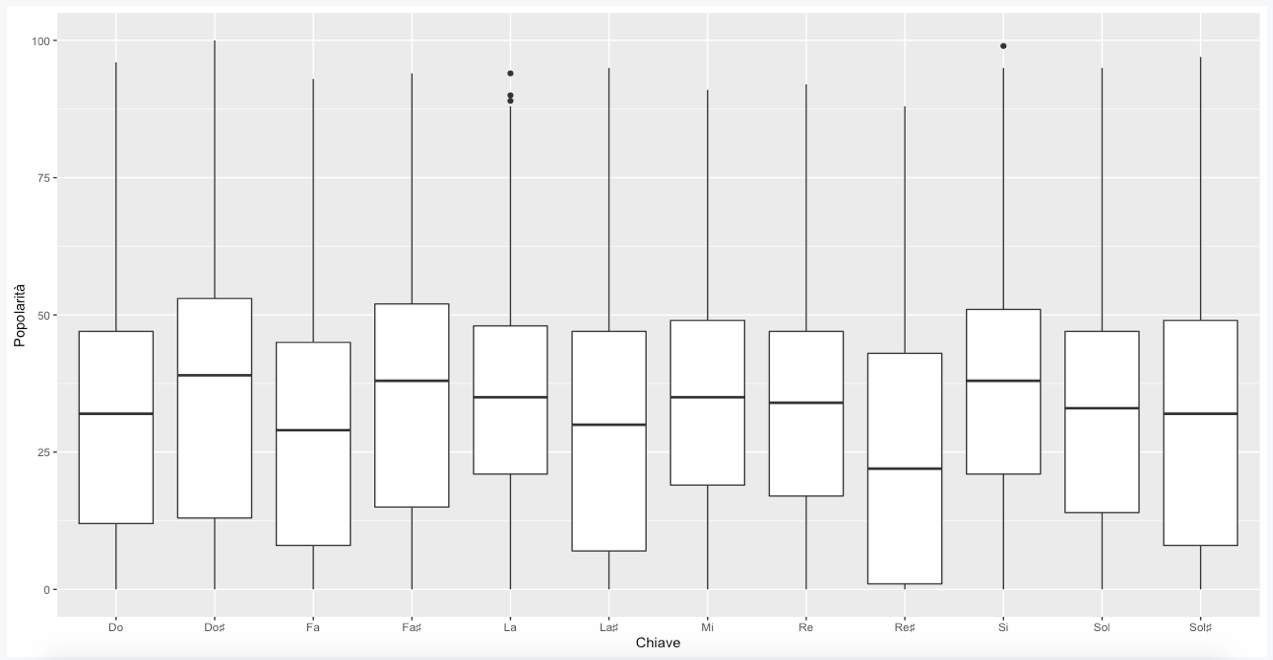
\includegraphics[width=1 \linewidth]{fig9.png}
    \caption{\textit{BoxPlot} condizionati per la visualizzazione delle distribuzioni condizionate di popolarità in base alla chiave globale.}
    \label{fig:fig9}
\end{figure}
%------------------------------------------------
\section{Analisi dei caratteri quantitativi}\label{cquant}
Tutte le rimanenti 11 variabili quantitative sono state esaminate in varie fasi:
\begin{itemize}
    \item calcolo delle statistiche descrittive di base, tra cui i principali momenti e quantili
    \item analisi della forma della distribuzione e confronto con una Normale
    \item stima intervallare della media della variabile - sempre con un livello di significatività $\alpha=0.05$ -, poiché, come già esposto per quanto riguarda la proporzione campionaria delle modalità qualitative, la sola stima puntuale derivata dal campione è dominata da una certa incertezza e mostra scarsa utilità
    \item analisi della significatività delle reciproche correlazioni lineari
\end{itemize}
Per evitare una descrizione prolissa del lavoro svolto, in questa Sezione verranno esposti soltanto i risultati riscontrati sulle variabili più interessanti.
\subsection*{Variabile \textit{Acousticness}}
Le statistiche descrittive sul livello di "acusticità" della traccia sono riassunte nella Tabella 1:
{\begin{table}[H]
\centering

\begin{tabular}[t]{lc}
\toprule
\midrule
\textbf{Minimo}&0\\
\textbf{1o Quartile}&0.0945\\
\textbf{Mediana}&0.492\\
\textbf{Media}&0.493\\
\textbf{3o Quartile}&0.888\\
\textbf{Massimo}&0.996\\
\textbf{Moda}&0.995\\
\textbf{Coeff. di Variazione}&0.764\\
\bottomrule
\end{tabular}
\caption{Statistiche descrittive calcolate sul livello di acusticità.}
\end{table}}
È possibile dedurre che la distribuzione sia asimmetrica. Tuttavia, la differenza quasi trascurabile fra media e mediana è indizio di uno scarso grado di deviazione dalla condizione di simmetria. Queste deduzioni sono confermate dal valore - positivo e basso - dell'indice di asimmetria: $\frac{m_3}{m_2^{3/2}}=0.009$.\\
La distribuzione di \textit{Acousticness} è, inoltre, platicurtica, perchè la propria curtosi è inferiore al valore dell'indice in condizione di normalità, ovvero 3: $\frac{m_4}{m_2^{2}}=1.386$. Questa caratteristica implica generalmente un inspessimento delle code ed un appiattimento della campana gaussiana. Tali peculiarità vengono ritrovate visualizzando la distribuzione dell'acusticità (Figura \ref{fig:fig11}).
\begin{figure}[H]
    \centering
    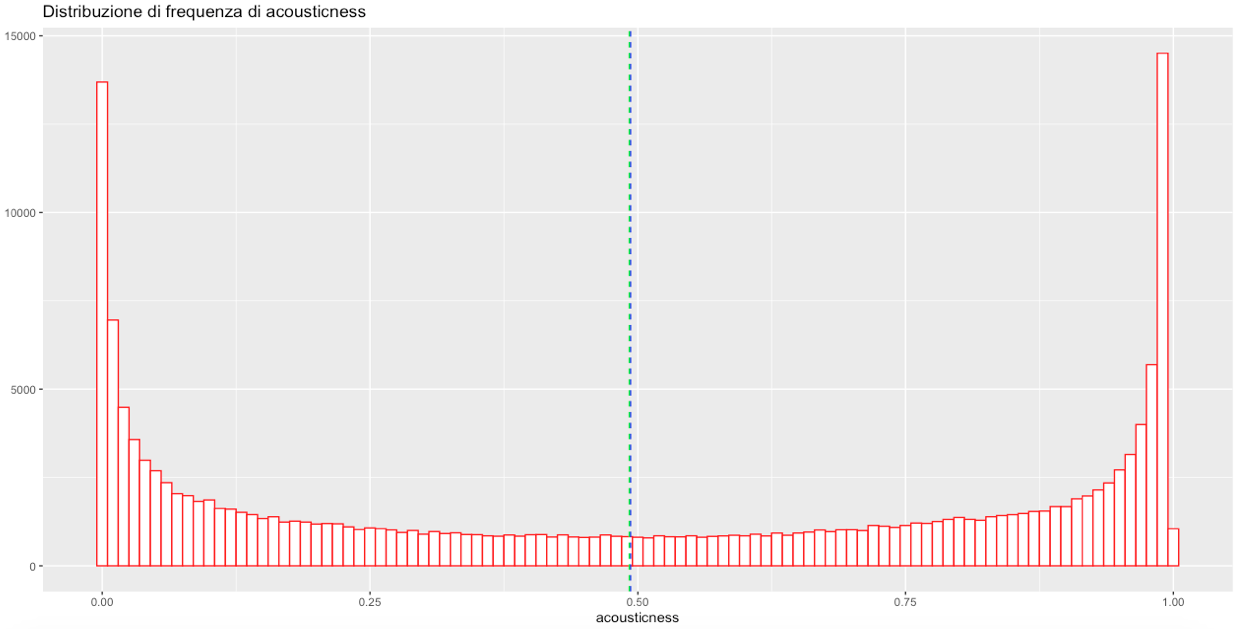
\includegraphics[width=1\linewidth]{fig11.png}
    \caption{Istogramma dell'acusticità. Le linee verticali tratteggiate corrispondono alla media (in blue) e alla mediana (in verde).}
    \label{fig:fig11}
\end{figure}
La forte deviazione dalla condizione Normale è suggerita anche dal grafico \textit{Quantile-Quantile} (Figura \ref{fig:fig12}), specialmente per quanto riguarda le code: quanto minore la somiglianza fra l'andamento dei punti corrispondenti ai quantili empirici e la retta associata alla distribuzione dei quantili teorici normali, tanto maggiore la differenza fra la variabile esaminata e la Gaussiana.
\begin{figure}[H]
    \centering
    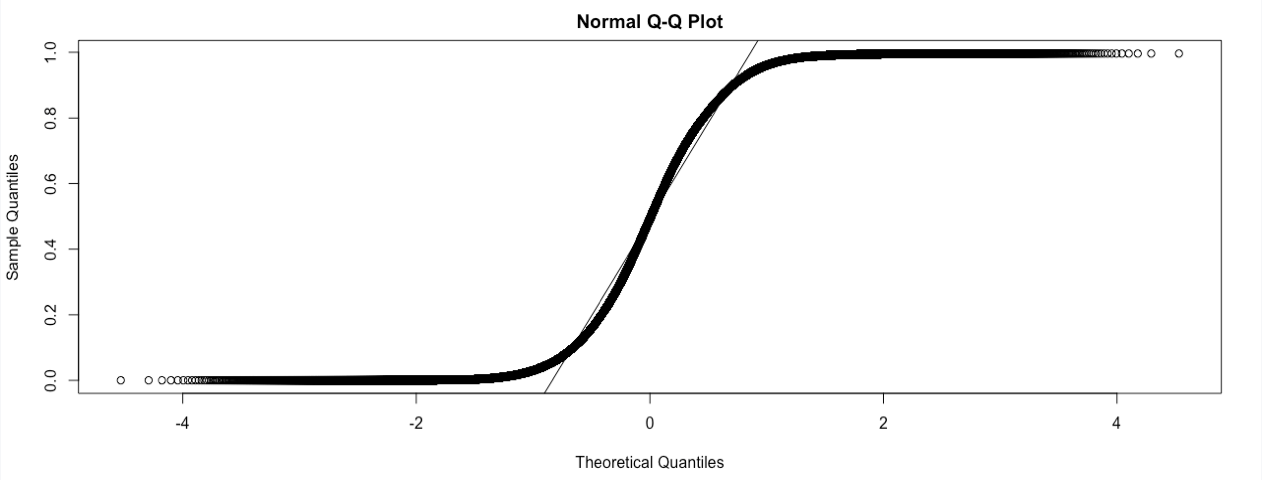
\includegraphics[width=1\linewidth]{fig12.png}
    \caption{Quantile-Quantile Plot per il confronto fra i quantili empirici e i quantili teorici.}
    \label{fig:fig12}
\end{figure}
Infine, con un livello di confidenza al 95\%, è possibile affermare che l'acusticità media sia contenuta nell'intervallo:
\begin{equation}
    (0.491, 0.495)
\end{equation}
Ciò significa che, generalizzando con confidenza al 95\%, le tracce musicali hanno in media una probabilità di essere completamente acustiche inferiore rispetto alla probabilità di includere strumenti elettronici, poichè l'intervallo di confidenza di "acousticness" ha estremo superiore minore di 0.5. 
\subsection*{Variabile \textit{Danceability}}
Le statistiche descrittive sul livello di ballabilità della traccia sono riassunte nella Tabella 2:
{\begin{table}[H]
\centering

\begin{tabular}[t]{lc}
\toprule
\midrule
\textbf{Minimo}&0\\
\textbf{1o Quartile}&0.417\\
\textbf{Mediana}&0.548\\
\textbf{Media}&0.538\\
\textbf{3o Quartile}&0.667\\
\textbf{Massimo}&0.988\\
\textbf{Moda}&0.565\\
\textbf{Coeff. di Variazione}&0.326\\
\bottomrule
\end{tabular}
\caption{Statistiche descrittive calcolate sul livello di ballabilità.}
\end{table}}
La ballabilità dei brani rivela una forma asimmetrica negativa, con un valore dell'indice di asimmetria pari a -0.213. Tale risultato indica che le frequenze più elevate della distribuzione tendono a disporsi su valori elevati di ballabilità, com'è ragionevole supporre, dato che le tracce musicali sono in gran parte concepite per essere accompagnate da qualche forma di ballo. L'allontanamento dalla normalità è molto lieve, di tipo platicurtico (come riscontrato in Figura \ref{fig:fig14}): la curtosi è, infatti, pari a 2.575.\\
\begin{figure}[H]
    \centering
    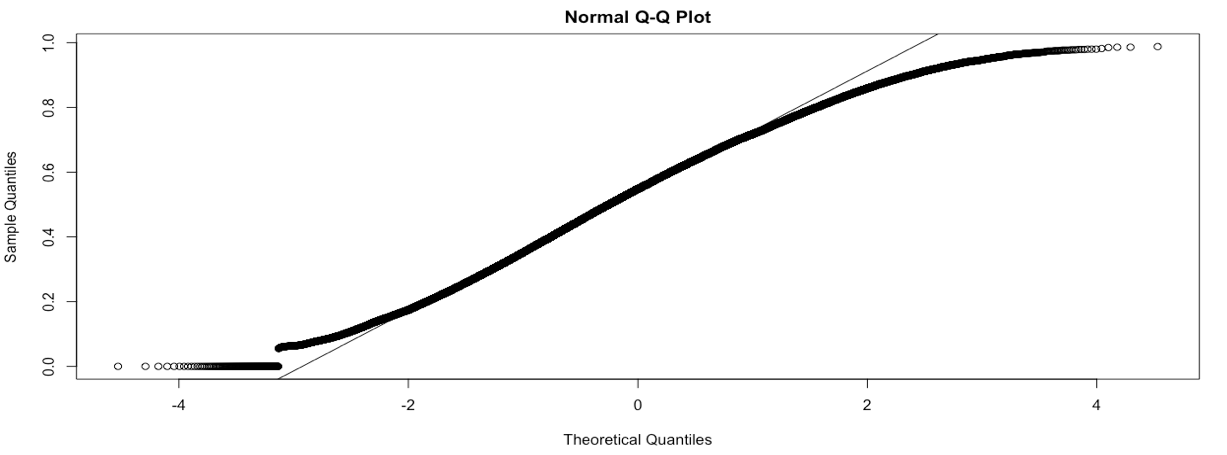
\includegraphics[width=1\linewidth]{fig14.png}
    \caption{Quantile-Quantile Plot per il confronto fra i quantili empirici e i quantili teorici.}
    \label{fig:fig14}
\end{figure}
In Figura \ref{fig:fig13} è visibile la forma della distribuzione della ballabilità.
\begin{figure}[H]
    \centering
    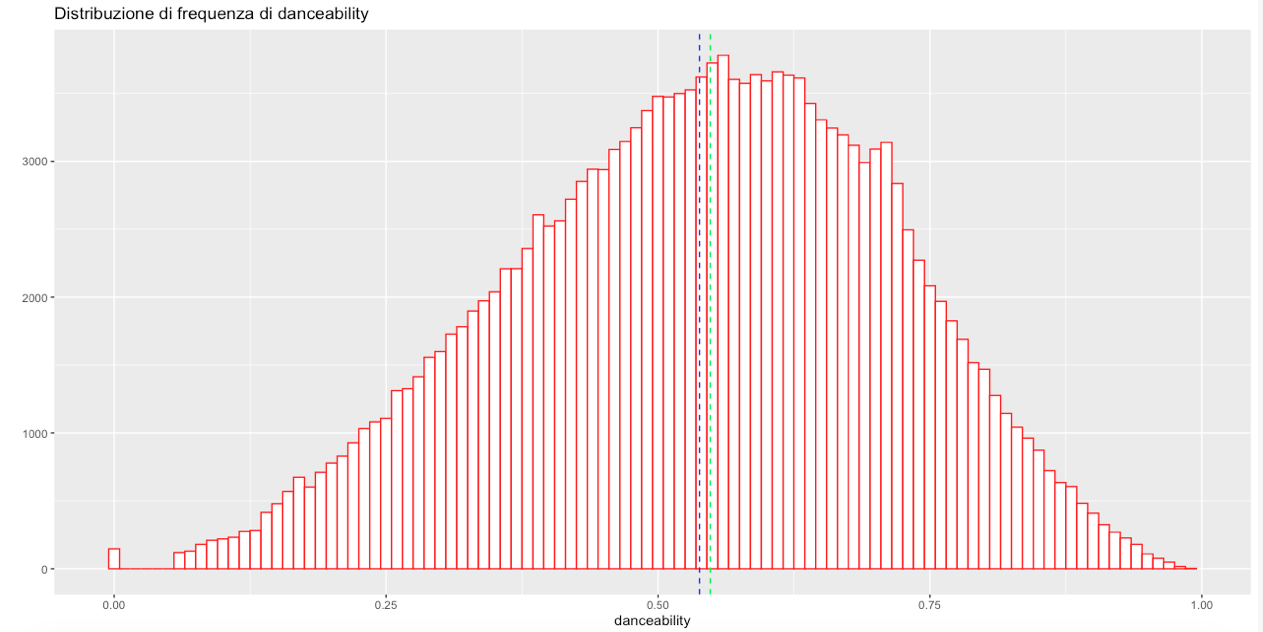
\includegraphics[width=1\linewidth]{fig13.png}
    \caption{Istogramma della ballabilità. Le linee verticali tratteggiate corrispondono alla media (in blue) e alla mediana (in verde).}
    \label{fig:fig13}
\end{figure}
La ballabilità media generale è stimata, con un livello di confidenza del 95\%, nel seguente intervallo:
\begin{equation}
    (0.537, 0.539)
\end{equation}
Si conclude che l'industria discografica preferisce produrre, in media, basi musicali che possano essere più facilmente accompagnate da una danza, ovvero con un livello di \textit{danceability} ben oltre lo 0.5.

\subsection*{Variabile \textit{Instrumentalness}}
Il grado di confidenza con cui si definisce "strumentale" la traccia è, innanzitutto, descritto dalle grandezze in Tabella 3:
{\begin{table}[H]
\centering

\begin{tabular}[t]{lc}
\toprule
\midrule
\textbf{Minimo}&0\\
\textbf{1o Quartile}&0\\
\textbf{Mediana}&0\\
\textbf{Media}&0.162\\
\textbf{3o Quartile}&0.087\\
\textbf{Massimo}&1\\
\textbf{Moda}&0\\
\textbf{Coeff. di Variazione}&1.91\\
\bottomrule
\end{tabular}
\caption{Statistiche descrittive calcolate sul livello di strumentalità.}
\end{table}}
Esso presenta, pertanto, una variabilità nettamente superiore rispetto alle variabili precedentemente esaminate, ed è caratterizzato da una forte asimmetria positiva - misurata pari a 1.682. La forma della distribuzione, descritta da un indice di curtosi superiore a 3 (4.119), è caratterizzata da un allontanamento dalla normalità di tipo leptocurtico: le code tendono ad assottigliarsi, spingengo verso l'alto le frequenze più elevate. Infatti, in Figura \ref{fig:fig15}, soltanto la coda di destra - per la forte asimmetria positiva - si presenta molto lunga ed estremamente sottile. Questa condizione viene riscontrata anche osservando il grafico \textit{Quantile-Quantile} in Figura \ref{fig:fig16}.
\begin{figure}[H]
    \centering
    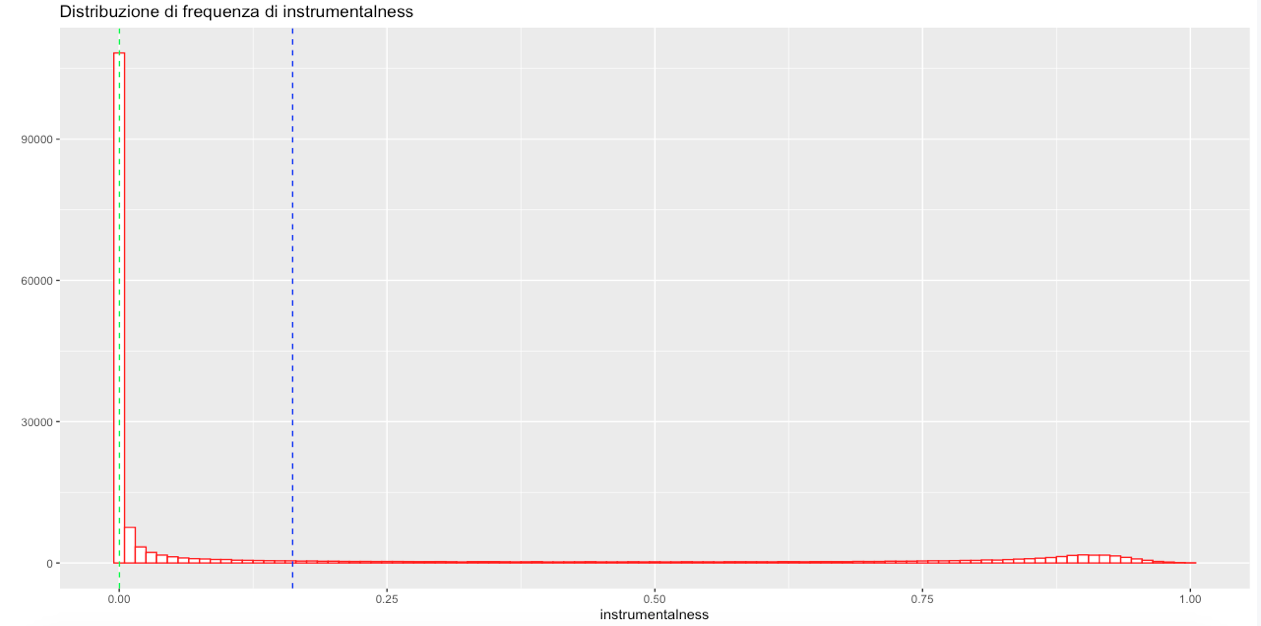
\includegraphics[width=1\linewidth]{fig15.png}
    \caption{Istogramma della \textit{instrumentalness}. Le linee verticali tratteggiate corrispondono alla media (in blue) e alla mediana (in verde).}
    \label{fig:fig15}
\end{figure}. 
\begin{figure}[H]
    \centering
    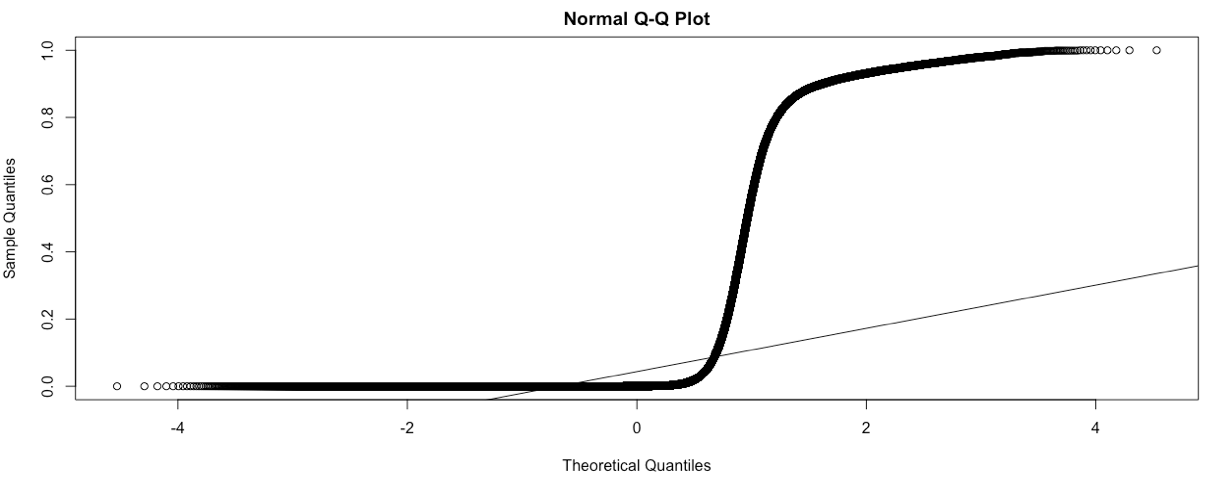
\includegraphics[width=1\linewidth]{fig16.png}
    \caption{Quantile-Quantile Plot per il confronto fra i quantili empirici e i quantili teorici.}
    \label{fig:fig16}
\end{figure}
Infine, la stima della quantità media di contenuto esclusivamente strumentale all'interno delle tracce, con un livello di confidenza del 95\%, è compreso nel seguente intervallo di confidenza:
\begin{equation}
    (0.16,0.163)
\end{equation}
È quindi ragionevole concludere - con confidenza al 95\% - che, in media, si tenda a produrre brani che contengono tra il 16 e il 16.3\% di parti strumentali.

\subsection*{Variabile \textit{Speechiness}}
Poichè nel paragrafo precedente si è dimostrato come la voce formi elemento tendenzialmente essenziale nella produzione di una traccia, è utile approfondire la variabile che distingue gli elementi vocali in "cantato" e "parlato", con un grado di \textit{speechiness} compreso fra 0 e 1. Le statistiche descrittive di base sono mostrate nella Tabella 4:
{\begin{table}[H]
\centering

\begin{tabular}[t]{lc}
\toprule
\midrule
\textbf{Minimo}&0\\
\textbf{1o Quartile}&0.0349\\
\textbf{Mediana}&0.045\\
\textbf{Media}&0.094\\
\textbf{3o Quartile}&0.075\\
\textbf{Massimo}&0.969\\
\textbf{Moda}&0.0347\\
\textbf{Coeff. di Variazione}&1.594\\
\bottomrule
\end{tabular}
\caption{Statistiche descrittive calcolate sul livello di \textit{speechiness}.}
\end{table}}
La variabilità tende ad essere ancora una volta elevata, e la distribuzione presenta un'asimmetria positiva di gran lunga superiore alle variabili precedenti: 4.236. L'elevatissimo valore di curtosi (22.375) indica che la forma della distribuzione è di tipo leptocurtico, come rilevato riguardo alla "strumentalità", ma con un ulteriore assottigliamento della coda destra (Figura \ref{fig:fig17} e \ref{fig:fig18}).
\begin{figure}[H]
    \centering
    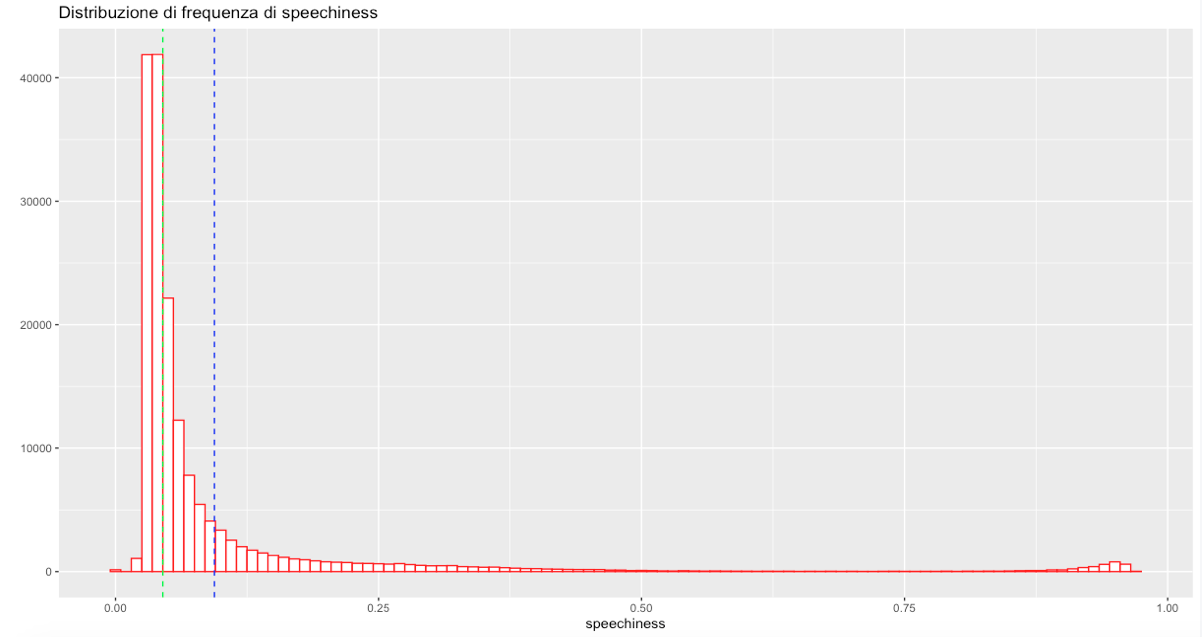
\includegraphics[width=1\linewidth]{fig17.png}
    \caption{Istogramma della \textit{speechiness}. Le linee verticali tratteggiate corrispondono alla media (in blue) e alla mediana (in verde).}
    \label{fig:fig17}
\end{figure}
\begin{figure}[H]
    \centering
    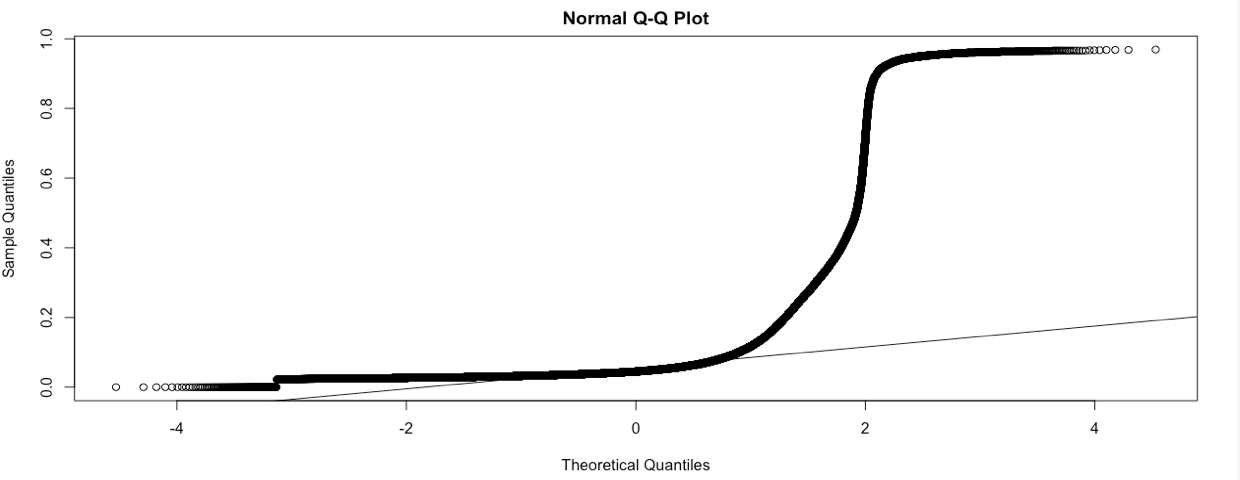
\includegraphics[width=1\linewidth]{fig18.png}
    \caption{Quantile-Quantile Plot per il confronto fra i quantili empirici e i quantili teorici.}
    \label{fig:fig18}
\end{figure}
Queste caratteristiche sono, in altre parole, manifestazione di una generale tendenza a preferire una base vocale cantata, piuttosto che simile ad un discorso, nonostante la grande diffusione di generi musicali come il \textit{rap}. Infatti, la probabilità media di rilevare del parlato all'interno delle canzoni è, comprensibilmente, molto bassa, stimata - con un livello di confidenza del 95\% - all'interno del seguente intervallo:
\begin{equation}
    (0.093, 0.095)
\end{equation}
ovvero tra il 9.3\% e il 9.5\%.

\subsection*{Variabile \textit{Liveness}}
Un altro carattere quantitativo interessante consiste nella probabilità che la traccia sia stata registrata durante un'esibizione dal vivo. Le statistiche descrittive sono riportate in Tabella 5:
{\begin{table}[H]
\centering

\begin{tabular}[t]{lc}
\toprule
\midrule
\textbf{Minimo}&0\\
\textbf{1o Quartile}&0.0984\\
\textbf{Mediana}&0.135\\
\textbf{Media}&0.207\\
\textbf{3o Quartile}&0.263\\
\textbf{Massimo}&1\\
\textbf{Moda}&0.111\\
\textbf{Coeff. di Variazione}&0.855\\
\bottomrule
\end{tabular}
\caption{Statistiche descrittive calcolate sul livello di \textit{liveness}.}
\end{table}}
La distribuzione è positivamente asimmetrica, con un indice pari a 2.146, e leptocurtica ($\frac{m_4}{m_2^{2}}=7.916$). La sua variabilità è moderata. In Figura \ref{fig:fig19}, è possibile notare la sottile coda di destra, specialmente per valori maggiori di 0.5, e l'elevata frequenza delle probabilità più ridotte, in un intervallo compreso fra 0 e, circa, 0.375. L'allontanamento dalla condizione di normalità è perfettamente descritto nel grafico \textit{Quantile-Quantile} (Figura \ref{fig:fig20}): anche qui, come nei due casi precedenti, i quantili empirici relativi alla coda destra sono estremamente distanti da quelli teorici.
\begin{figure}[H]
    \centering
    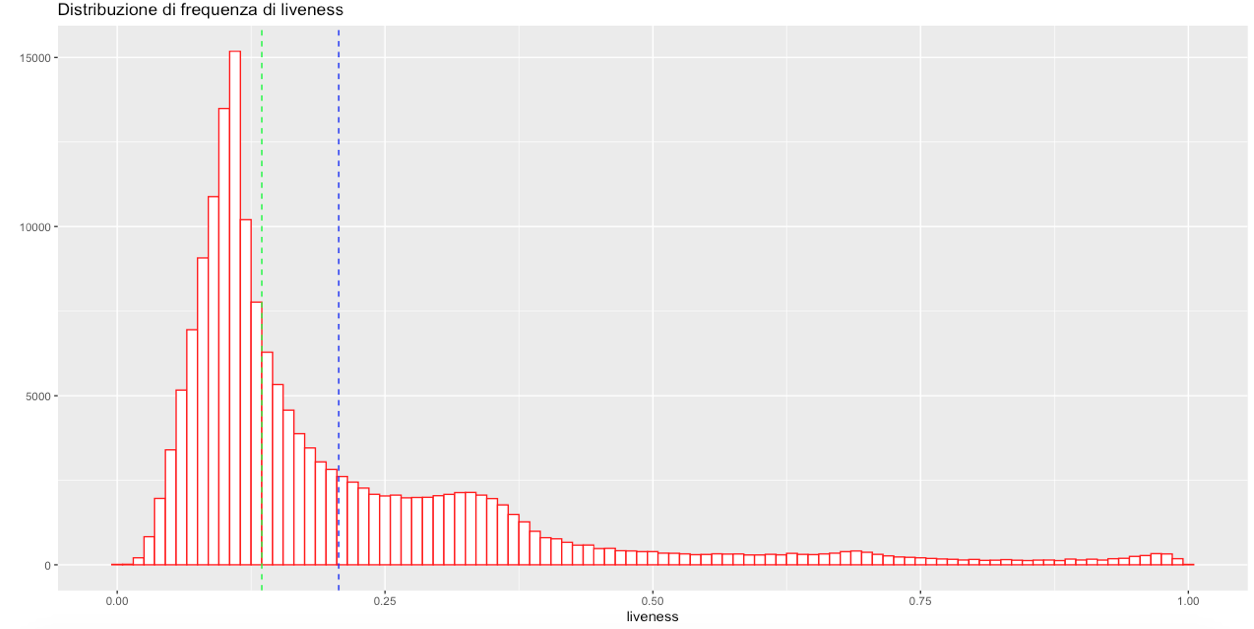
\includegraphics[width=1\linewidth]{fig19.png}
    \caption{Istogramma della \textit{liveness}. Le linee verticali tratteggiate corrispondono alla media (in blue) e alla mediana (in verde).}
    \label{fig:fig19}
\end{figure}
\begin{figure}[H]
    \centering
    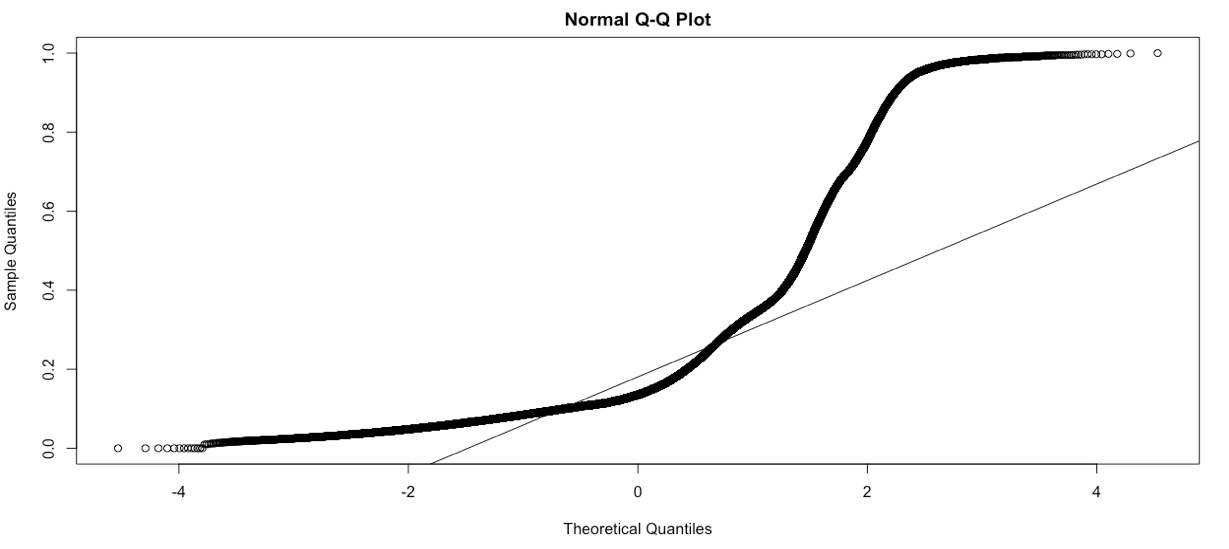
\includegraphics[width=1\linewidth]{fig20.png}
    \caption{Quantile-Quantile Plot per il confronto fra i quantili empirici e i quantili teorici.}
    \label{fig:fig20}
\end{figure}
Infine, è possibile affermare, con confidenza al 95\%, che la probabilità media che la traccia sia stata registrata dal vivo sia compresa nell'intervallo
\begin{equation}
    (0.206, 0.208)
\end{equation}

\subsection*{Variabile \textit{Valence}}
La variabile che registra la positività percepita durante l'ascolto del brano è caratterizzata dalle seguenti  statistiche di base (Tabella 6):
{\begin{table}[H]
\centering

\begin{tabular}[t]{lc}
\toprule
\midrule
\textbf{Minimo}&0\\
\textbf{1o Quartile}&0.322\\
\textbf{Mediana}&0.544\\
\textbf{Media}&0.532\\
\textbf{3o Quartile}&0.749\\
\textbf{Massimo}&1\\
\textbf{Moda}&0.961\\
\textbf{Coeff. di Variazione}&0.493\\
\bottomrule
\end{tabular}
\caption{Statistiche descrittive calcolate sul livello di positività.}
\end{table}}
La distribuzione presenta una leggera asimmetria negativa (-0.124) e una forma platicurtica - la curtosi è 1.949 -, come osservato in Figura \ref{fig:fig21}. 
\begin{figure}[H]
    \centering
    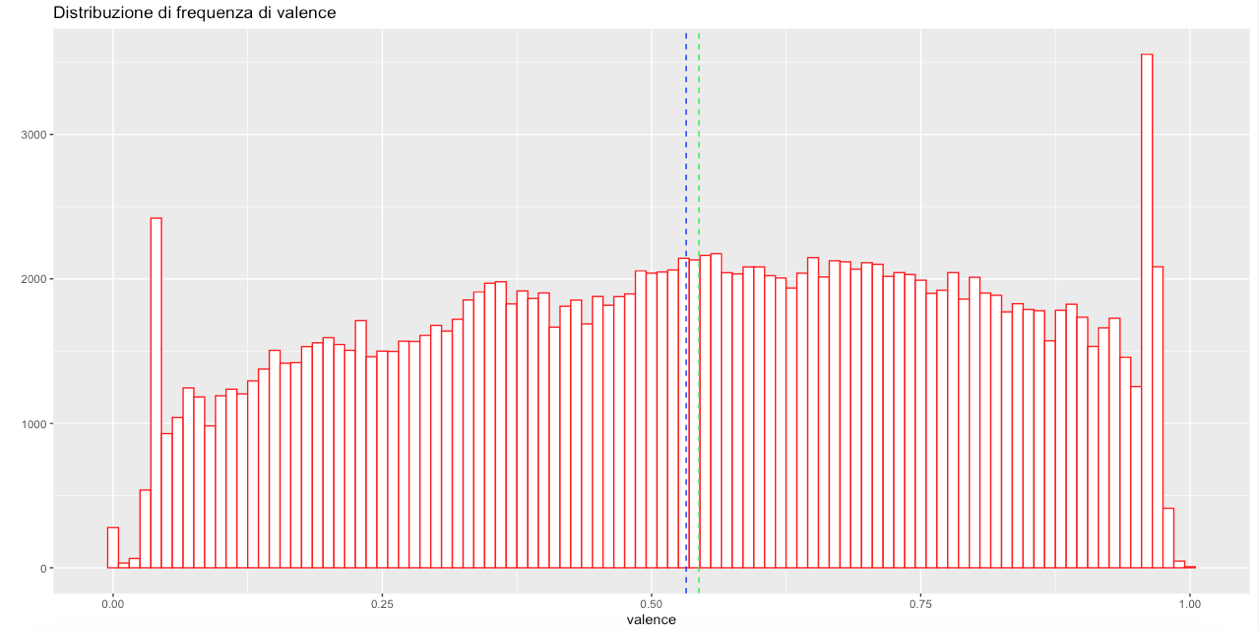
\includegraphics[width=1\linewidth]{fig21.png}
    \caption{Istogramma della positività trasmessa dal brano. Le linee verticali tratteggiate corrispondono alla media (in blue) e alla mediana (in verde).}
    \label{fig:fig21}
\end{figure}
Le code spesse deformano la tipica forma a campana verso una densità visibilmente più piatta. Questa anomalia è riscontrabile in Figura \ref{fig:fig22}.
\begin{figure}[H]
    \centering
    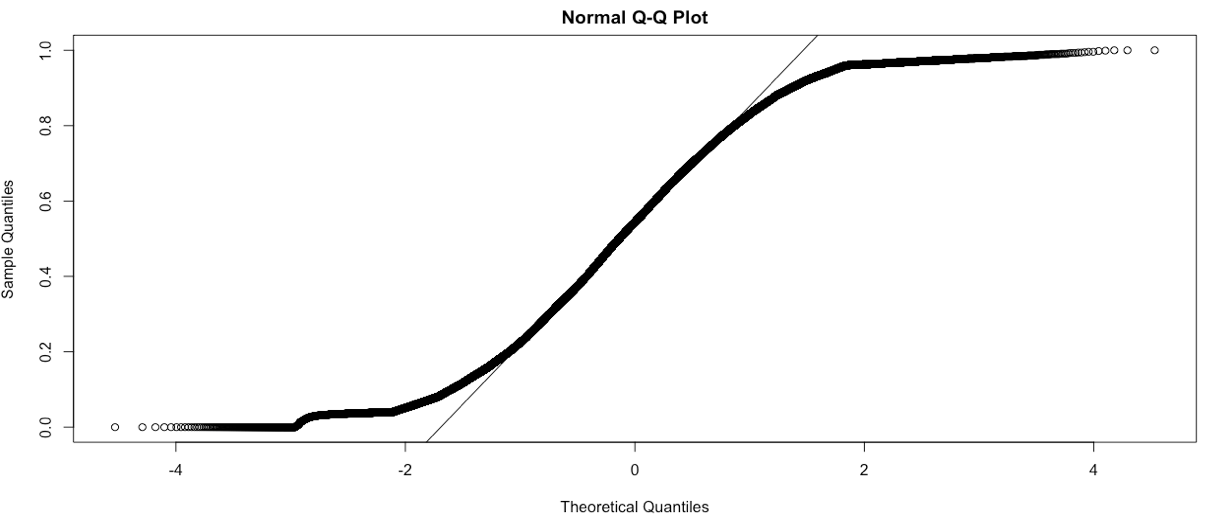
\includegraphics[width=1\linewidth]{fig22.png}
    \caption{Quantile-Quantile Plot per il confronto fra i quantili empirici e i quantili teorici.}
    \label{fig:fig22}
\end{figure}
Il livello emotivo, pertanto, si distribuisce in maniera bilanciata: la produzione musicale, nelle proprie numerose declinazioni di genere, è in grado di esprime qualsiasi tipo di stato d'animo, dal più negativo - quando \textit{valence} è nulla - al più positivo - quando la colonna assume valore 1, senza essere dominata da nessuna delle due polarità. Tuttavia, con confidenza al 95\%, è possibile affermare che l'industria discografica propenda leggermente verso un sentimento più positivo, poiché il livello emotivo medio è stimato all'interno dell'intervallo
\begin{equation}
    (0.531, 0.533)
\end{equation}
\\
Si è proceduto, poi, a verificare l'esistenza di qualche tipo di connessione statistica fra il livello emotivo e altre variabili qualitative. Innanzitutto, si è deciso di studiare il legame fra il decennio di pubblicazione e la positività trasmessa, per estrarre evidenze sul fatto che i contenuti musicali risentano del periodo storico non solo da un punto di vista stilistico, ma anche da un punto di vista dei sentimenti espressi. Pertanto, è stato eseguito un test del Chi-quadrato sulla relazione fra \textit{Valence} e \textit{Decade}, con 1 grado di libertà, supponendo una reciproca indipendenza fra le varie decadi. Fissato un livello di significatività del 5\%, s'ottiene un \textit{pvalue} inferiore alla soglia, rifiutando l'ipotesi di indipendenza. Viene anche rifiutata l'ipotesi di uguaglianza dei livelli emotivi medi per ogni decennio, tramite test ANOVA con $\alpha=0.05$ e 10 gradi di libertà, confermando ulteriormente l'esistenza di una relazione fra i due fenomeni. In Figura \ref{fig:fig23}, è possibile distinguere le differenti distribuzioni della positività per gruppo. 
\begin{figure}[H]
    \centering
    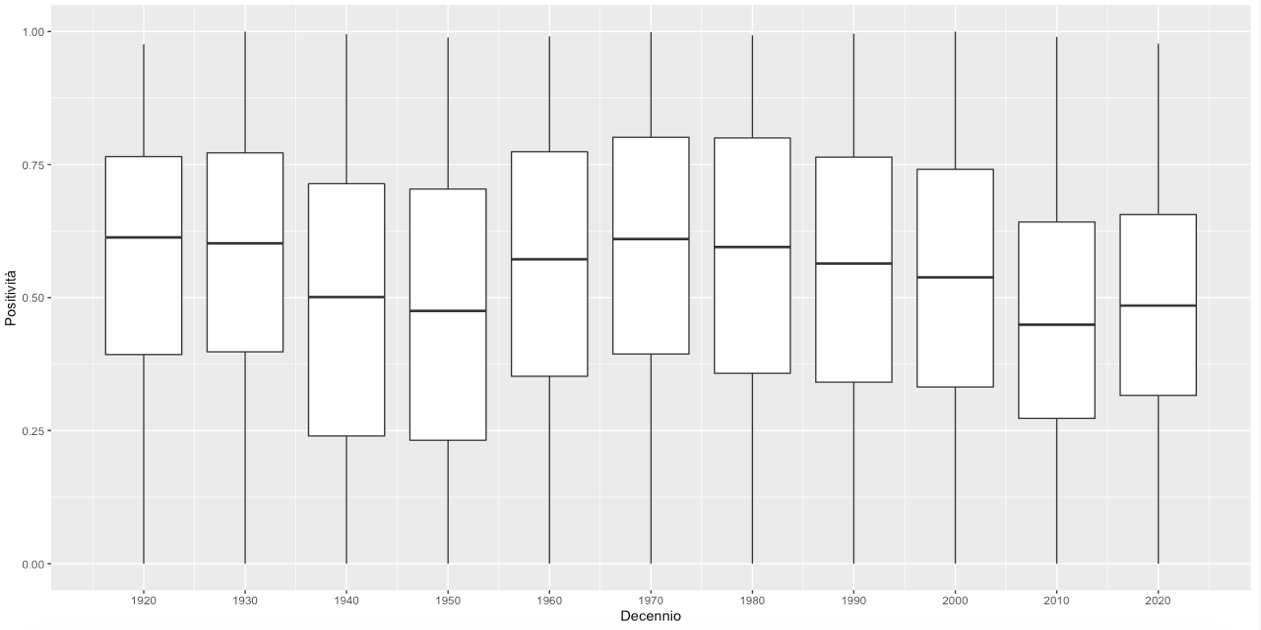
\includegraphics[width=1 \linewidth]{fig23.png}
    \caption{\textit{BoxPlot} condizionati per la visualizzazione delle distribuzioni condizionate di positività in base al decennio esaminato.}
    \label{fig:fig23}
\end{figure}
Nella stessa maniera, vengono esaminate le dipendenze della positività rispetto alla tonalità e alla chiave del brano, ipotizzando che gli elementi tecnici di base possano influenzare il sentimento della traccia finale. In entrambi i casi, l'ipotesi di indipendenza viene rifiutata tramite calcolo dell'indice di connessione $\chi^2$ con livello di significatività 0.05, e così anche l'ipotesi di uguaglianza delle medie di \textit{Valence} rispetto a entrambi i fattori condizionanti - test ANOVA -, sempre con confidenza al 95\%.

\subsection*{Variabile \textit{Popularity}}
La popolarità è associata alle seguenti statistiche (Tabella 6):
{\begin{table}[H]
\centering
\begin{tabular}[t]{lc}
\toprule
\midrule
\textbf{Minimo}&0\\
\textbf{1o Quartile}&12\\
\textbf{Mediana}&33\\
\textbf{Media}&31.56\\
\textbf{3o Quartile}&48\\
\textbf{Massimo}&100\\
\textbf{Moda}&0\\
\textbf{Coeff. di Variazione}&0.684\\
\bottomrule
\end{tabular}
\caption{Statistiche descrittive calcolate sul livello di popolarità.}
\end{table}}
La moda viene individuata in corrispondenza di 0: il grado di popolarità su \textit{Spotify} più diffuso all'interno del campione esaminato è quello nullo, coprendo addirittura fino al 16.1\% delle osservazioni totali. La variabilità è bassa e la distribuzione rivela un discreto indice di asimmetria negativo, pari a -0.021, e un forma moderatamente platicurtica (Figura \ref{fig:fig25}), con curtosi uguale a 1.985. Osservando la Figura \ref{fig:fig24}, è possibile notare, senza considerare il valore di moda, come le misure più frequenti siano concentrate nell'intervallo 25-50.
\begin{figure}[H]
    \centering
    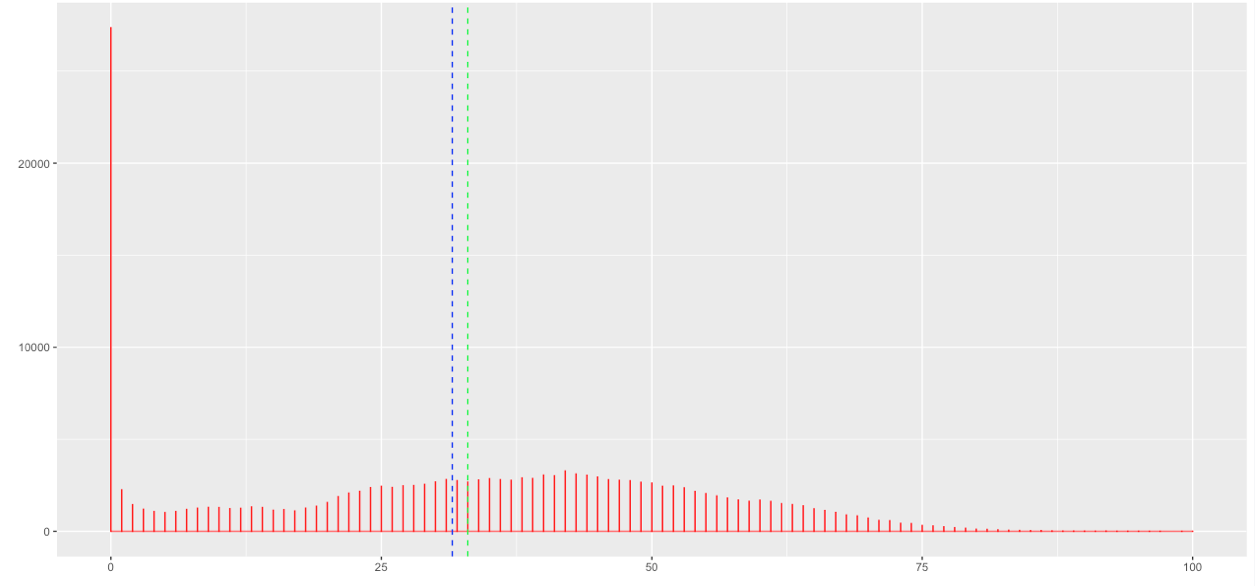
\includegraphics[width=1\linewidth]{fig24.png}
    \caption{Istogramma della popolarità. Le linee verticali tratteggiate corrispondono alla media (in blue) e alla mediana (in verde).}
    \label{fig:fig24}
\end{figure}
\begin{figure}[H]
    \centering
    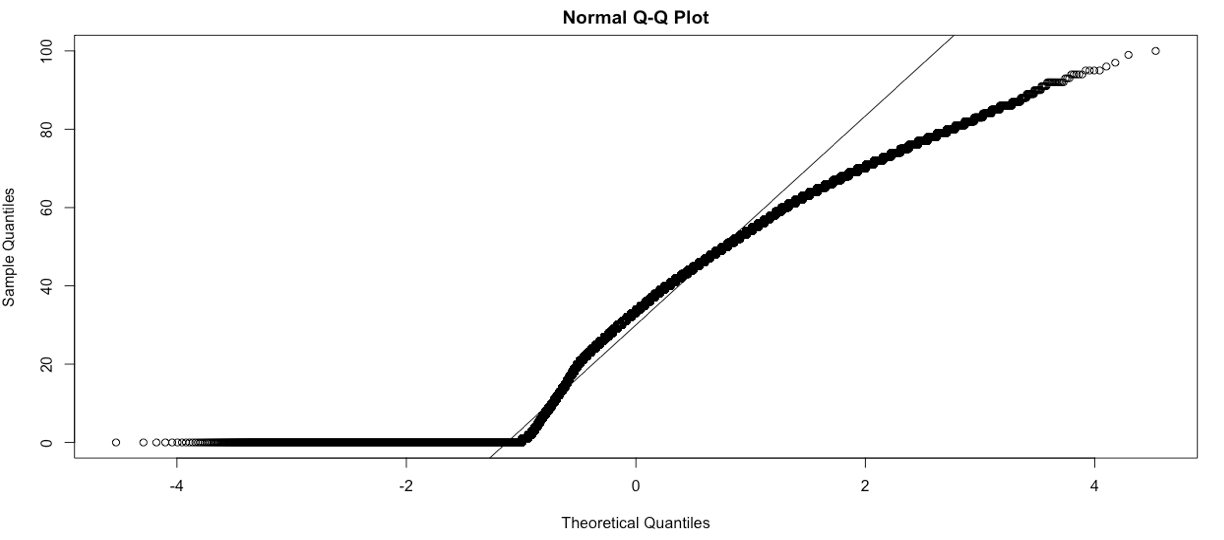
\includegraphics[width=1\linewidth]{fig25.png}
    \caption{Quantile-Quantile Plot per il confronto fra i quantili empirici e i quantili teorici.}
    \label{fig:fig25}
\end{figure}
\subsection{Correlazioni lineari}\label{corr}
Successivamente, sono stati stimati i coefficienti di correlazione di Pearson per tutte le possibili coppie di variabili quantitative, effettuando il corrispettivo test con livello di confidenza fissato al 95\%, per valutare la significatività statistica dei valori $\rho$. Il grado di reciproca dipendenza lineare fra i vari caratteri è visibile in Figura \ref{fig:fig26}.
\begin{figure}[H]
    \centering
    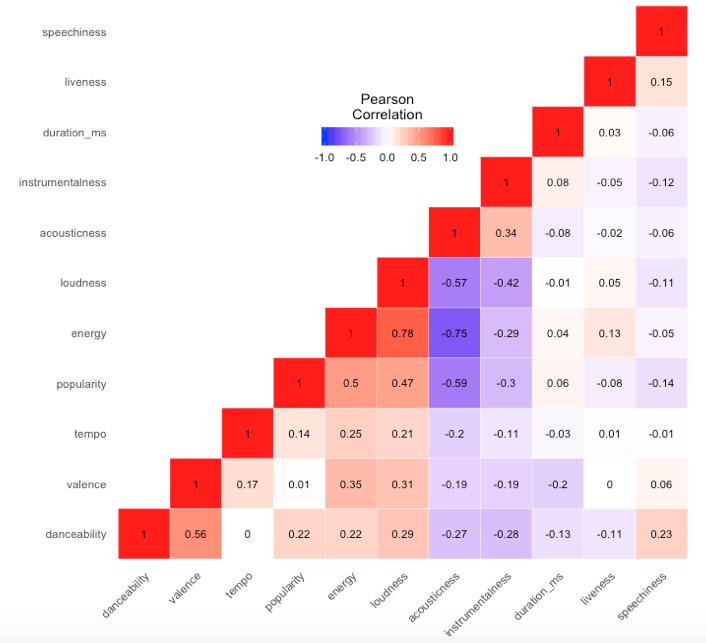
\includegraphics[width=1\linewidth]{fig26.png}
    \caption{\textit{Heatmap} per la visualizzazione dei coefficienti di correlazione lineare di Pearson fra tutte le variabili quantitative.}
    \label{fig:fig26}
\end{figure}
L'unica correlazione lineare statisticamente non significativa ad un livello di confidenza del 95\% viene riscontrata fra \textit{liveness} e positività: il \textit{pvalue} è 0.86.\\
I valori $\rho$ più rilevanti possono essere riscontrati fra le seguenti coppie di fenomeni:
\begin{itemize}
    \item energia e volume: $\rho=0.78$ 
    \item energia e "acusticità": $\rho=-0.75$
    \item popolarità e "acusticità: $\rho=-0.59$, per cui i brani con strumenti elettronici attrarrebbero maggiori ascolti
    \item volume e "acusticità": $\rho=-0.57$, per cui all'assenza di strumenti elettronici si associa un minor livello di decibel
    \item ballabilità e \textit{valence}: $\rho=0.56$, per cui maggiore la positività percepita dall'ascolto di un brano, maggiore la facilità ad associargli una danza, e viceversa. 
\end{itemize}
In fase di costruzione di un modello di regressione lineare, sarà necessario valutare queste collinearità fra le colonne della matrice del disegno, poiché potrebbero penalizzare la corretta stima dei coefficienti di regressione.
%------------------------------------------------
\section{Regressione lineare semplice}
Appurata l’esistenza di legami lineari statisticamente significativi fra il grado di popolarità di una traccia - considerato in questa fase come variabile dipendente - e molte delle altre colonne disponbili - variabili indipendenti -, si pone un vincolo di linearità sulla forma funzionale del modello che possa descrivere tali relazioni, ricercando, dunque, la retta ottimale in termini di Errore Quadratico Medio (MSE).\\
In particolare, il modello di regressione lineare semplice è specificato dalla seguente relazione:
\begin{equation}
    y_i=f(x_i;\beta)+\in_i
\end{equation}
dove $\in_i$ è l'errore casuale e $f(x_i;\beta)$ è la funzione che combina i valori delle variabili indipendenti e i rispettivi coefficienti di regressione per determinare l'osservazione $y_i$. In questa Sezione, verranno stimati modelli univariati caratterizzati da una funzione $f(x_i;\beta)$ di primo grado.\\
È opportuno specificare che l'eccessiva differenza di scala fra alcune variabili ha reso necessaria una mappatura di tutti i caratteri quantitativi fra 0 e 1, in quanto, altrimenti, le stime dei coefficienti di regressione non sarebbero state confrontabili, dunque inutili per l'obiettivo del progetto. Questa operazione ha implicato l'uso di una trasformazione in grado di mantenere inalterata la forma della distribuzione e gestire valori negativi:
\begin{equation}
    X_i'=\frac{X_i-X_{\text{min}}}{X_{\text{max}}-X_{\text{min}}}
\end{equation}
con $X_{\text{min}}$ e $X_{\text{max}}$ rispettivamente il massimo e il minimo della colonna X. Si è inoltre deciso di convertire le variabili qualitative in tipo \texttt{factor}, in modo che ogni loro modalità potesse essere considerata come una colonna \textit{dummy}, e potesse essere quindi possibile estrarre l'influenza di ciascuna classe al netto delle altre.\\
La significatività statistica dei coefficienti di regressione di ciascun modello è stata verificata mediante test $t$ con un livello di significatività $\alpha=0.05$, mentre la bontà di adattamento è stata valutata mediante coefficiente di determinazione $R^2$.
I risultati di ciascuna prova sono riassunti come segue.
\subsection*{Popolarità $\sim$ Positività}
Data $P$, variabile del grado di popolarità, e $V$, positività trasmessa, il modello stimato è
\begin{equation}
    P=0.311484+0.007671\bullet V
\end{equation}
Il test $t$ rifiuta l'ipotesi nulla per quanto riguarda sia l'intercetta che il coefficiente angolare, producendo un \textit{pvalue} estremamente basso nel primo caso e moderatamente basso nel secondo. Il coefficiente angolare $\beta_1$ mostra che, ad un aumento di un'unità percentuale del livello di positività trasmessa, la popolarità cresce, al netto dell'intercetta, di circa uno 0.008\%. Nonostante la significatività statistica del coefficiente di regressione, la capacità di tale modello di descrivere la variabilità della popolarità rimane molto scarsa: $R^2<0.001$.
\subsection*{Popolarità $\sim$ Chiave}
Data $P$, variabile del grado di popolarità, il modello ottenuto include i seguenti parametri $\beta$ - con stime approssimate al secondo decimale per esigenze di leggibilità:
{\begin{table}[H]
\centering
\begin{tabular}[t]{lcc}
\toprule
&Parametro&PValue\\
\midrule
\textbf{Intercetta}&0.31&0\\
\textbf{Do\#}&0.04&0\\
\textbf{Re}&0.01&0\\
\textbf{Re\#}&-0.06&0\\
\textbf{Mi}&0.02&0\\
\textbf{Fa}&-0.02&0\\
\textbf{Fa\#}&0.04&0\\
\textbf{Sol}&0.005&0.02\\
\textbf{Sol\#}&-0.002&0.37\\
\textbf{La}&0.02&0\\
\textbf{La\#}&-0.016&0\\
\textbf{Si}&0.04&0\\
\bottomrule
\end{tabular}
\end{table}}
La stima del coefficiente di regressione della chiave di "Sol" è positiva ma associata ad una bassa significatività statistica: il \textit{pvalue} è di poco inferiore ad $\alpha$. Il coefficiente di regressione della chiave di "Sol\#" è, invece, non significativo: non vi è evidenza di alcuna relazione lineare fra l'uso di tale chiave in fase di composizione del brano e il livello di popolarità. Tutte le altre stime sono altamente significative - il \textit{pvalue} tende ad essere nullo -, ma è possibile operare una distinzione. Infatti, le chiavi di "Do\#", "Re", "Mi", "Fa\#", "La" e "Si" hanno un'influenza positiva sulla popolarità: il loro uso permette di incrementare il grado della variabile dipendente, da una variazione minima dell'1\% (con "Re") ad un incremento massimo del 4\% ("Do\#" e "Fa\#"). Al contrario, le chiavi di "Re\#", "Fa" e "La\#" si rivelano fattori penalizzanti, con un decremento di popolarità che va dall'1\% al 6\%. In generale, la bontà di adattamento del modello è ancora scarsa: $R^2=0.013$.

\subsection*{Popolarità $\sim$ Decennio}
I coefficienti di regressione associati a ciascun decennio sono, ad un livello di confidenza del 95\%, tutti altamente significativi, tranne il parametro relativo agli anni '40. È possibile confermare quanto ipotizzato nella Sezione \ref{year}: l'influenza esercitata dalla modalità di decennio sulla popolarità è sempre positiva - i $\beta$ sono tutti maggiori di 0 -, ma la dimensione dell'incremento - ovvero il valore di tali parametri - cresce in ordine cronologico (Figura \ref{fig:figu}).
\begin{figure}[h]
    \centering
    \includegraphics[width=1\linewidth]{figu.png}
    \caption{Le stime dei coefficienti di regressione per decennio seguono un ordine cronologico crescente.}
    \label{fig:figu}
\end{figure}

\subsection*{Popolarità $\sim$ Tonalità}
Data P, popolarità del brano, il modello stimato è:
\begin{equation}
    P=0.3266221-0.0156036\bullet\text{Tonalità maggiore}
\end{equation}
Perciò, la scelta di una tonalità maggiore penalizza il valore della variabile dipendente, abbassando di circa l'1.6\% il grado di popolarità del brano.
%------------------------------------------------
\section{Regressione lineare multipla}
I modelli multivariati includono, invece, due o più variabili indipendenti per prevedere il valore della $Y$. I coefficienti di regressione rappresentano, quindi, le stime delle variazioni attese della variabile dipendente associate ad una variazione unitaria della singola $x_j$, mantenendo fisso tutto il resto del modello, quindi al netto degli altri predittori.\\
I successivi paragrafi esporranno i risultati ottenuti dalla costruzione di modelli lineari multivariati per la previsione del grado di popolarità del brano e del livello di positività da esso trasmesso. La significatività statistica della relazione fra le variabili dipendenti e l'insieme dei predittori è verificata mediante test $F$, cui ipotesi nulla nega l'esistenza di tale dipendenza lineare e ipotesi alternativa conferma il legame con almeno un regressore. La bontà di adattamento è stata valutata mediante il coefficiente di determinazione multiplo $R^2$ e la sua versione corretta, per evitare di sovrastimare la capacità del modello. 
\subsection{Previsione di \textit{Popularity}}
Innanzitutto, viene regredita la variabile \textit{popularity} sull'insieme totale di caratteri quantitativi. I coefficienti di regressione vengono stimati, con livello di confidenza al 95\%, tutti altamente significativi, eccetto il parametro associato alla durata del brano, che non appare pertanto utile per prevedere il grado di diffusione di un brano. Gli unici coefficienti con segno negativo sono relativi ad acusticità (-0.23), presenza di parti esclusivamente strumentali (-0.07), \textit{liveness} (-0.08), presenza di parlato \textit{speechiness} (-0.25) e positività (-0.23). Pertanto, sono da ritenersi più popolari le tracce che contengono strumenti elettronici - hanno dunque bassa \textit{acousticness} -, prive di parti strumentali, registrate in studio, prive di "parlato" e con un sentimento tendente verso una polarità negativa. Al contrario, i fenomeni con il maggior impatto positivo sulla $Y$ sono la ballabilità (0.27), il volume complessivo (0.21) e l'energia (0.11). Eseguendo un test $F$ con $\alpha=0.05$, viene rifiutata l'ipotesi di incorrelazione fra la popolarità e il set di caratteri quantitativi. Il coefficiente di determinazione multiplo è abbastanza buono (0.46), ed è pari alla propria versione corretta, indice del fatto che la capacità del modello non viene sopravvalutata.\\
Come visto nella Sezione \ref{corr}, molte delle variabili incluse nella matrice del disegno sono risultate fortemente correlate. È dunque necessario verificare che il modello appena stimato non sia affetto da problemi di multicollinearità, che possano penalizzarne la correttezza. Questa operazione è possibile grazie all'indice \textit{Variance Inflation Factor (VIF)}, il quale fornisce, per ciascun regressore, l'incremento subito dalla varianza della stima di $\beta$ rispetto alla condizione di perfetta incorrelazione fra le variabili indipendenti. Considerando una soglia pari a 4, la variabile "energia" risulta affetta da un moderato problema di collinearità. Risultava, infatti, essere il fenomeno associato ai più elevati valori di correlazione. L'energia viene pertanto rimossa dal set di candidati esplicativi.\\
Dopo la rimozione, il coefficiente di regressione associato al volume raggiunge un valore quasi doppio rispetto alla stima precedente (0.38), confermandosi come fattore quantitativo di maggior influenza sulla popolarità della traccia. L'$R^2$, invece, rimane quasi invariato.\\
Tale modello è stato infine integrato con le variabili qualitative della chiave, tonalità, presenza di contenuto esplicito e decennio. Le modalità di quest'ultima variabile sono associate a coefficienti molto elevati e tutti altamente significativi. Soltanto due delle classi della chiave, invece, vengono ritenute significativamente correlate alla variabile dipendente. I caratteri quantitativi, esclusa l'energia a priori, sono altamente significativi, ma le stime sono nettamente inferiori rispetto a quelle relative ai decenni. L'introduzione di \textit{Decade} ha pertanto ridimensionato la relativa importanza di tutti gli altri regressori, elevando, però, il coefficiente di determinazione multiplo: $R^2=0.79$, pari alla propria versione corretta. Il test $F$ rifiuta l'ipotesi nulla con un livello di confidenza del 95\%, ribadendo l'evidenza di un forte legame lineare fra \textit{popularity} e il set di predittori. Infine, il calcolo del \textit{VIF} verifica l'assenza di problemi di multicollinearità nella matrice del disegno.\\
Tuttavia, in Figura \ref{fig:29} e \ref{fig:fig30} è possibile individuare due caratteristiche negative dei residui di regressione ottenuti dall'ultimo modello stimato: l'eteroschedasticità - dato che, come si osserva, le previsioni sui valori più elevati sono associate a residui più variabili - e la distribuzione dei quantili abbastanza differente rispetto alla Normale.
\begin{figure}[h]
    \centering
    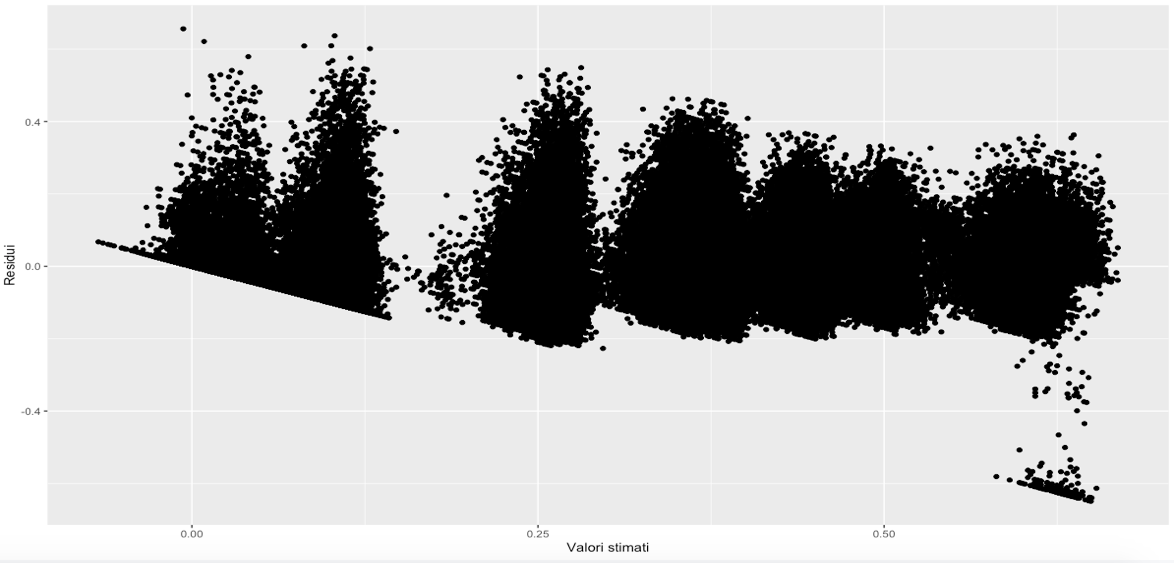
\includegraphics[width=1\linewidth]{fig29.png}
    \caption{\textit{Scatter plot} dei residui sui valori stimati dal modello.}
    \label{fig:fig29}
\end{figure}
\begin{figure}[h]
    \centering
    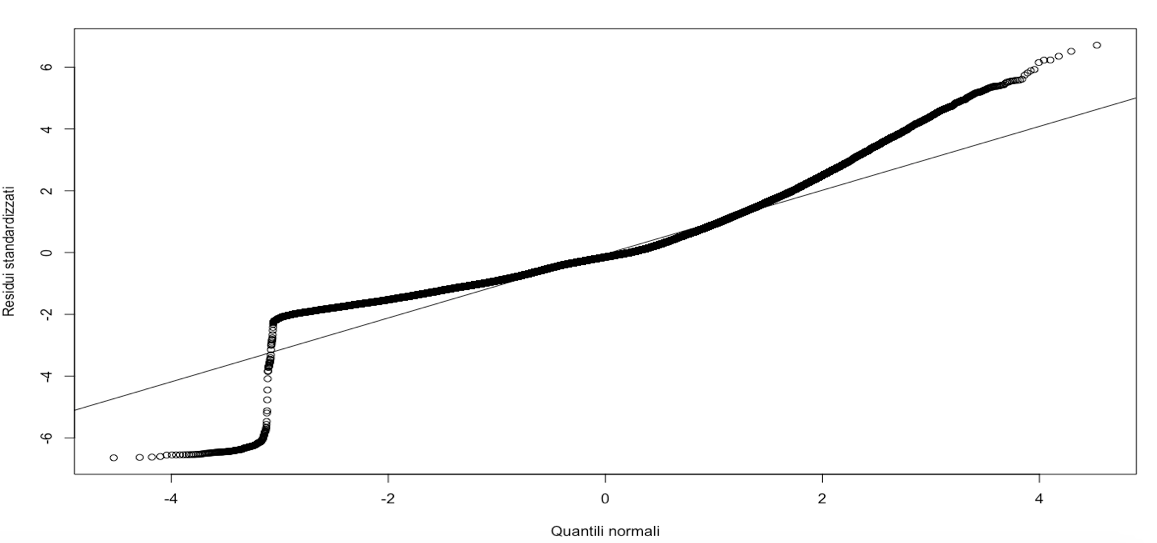
\includegraphics[width=1\linewidth]{fig30.png}
    \caption{Grafico \textit{Quantile-Quantile} per la valutazione della normalità dei residui.}
    \label{fig:fig30}
\end{figure}

\subsection{Previsione di \textit{Valence}}
Allo stesso modo, è stato stimato un modello che potesse prevedere il livello di positività trasmesso dal brano tramite il volume, l'energia, il tempo, la ballabilità, il decennio di pubblicazione, la tonalità e la chiave. Tramite test $F$, si rifiuta, con $\alpha=0.05$, l'ipotesi di incorrelazione fra la variabile dipendente e l’insieme dei regressori. Il volume risulta, tuttavia poco significativo - il \textit{pvalue} è 0.03 -, così come alcune modalità della chiave. I decenni sono associati a parametri negativi, eccezion fatta per gli anni '30, e ordinati, stavolta, in ordine cronologico decrescente. Ciò implica che, col passare del tempo, il sentimento tendenziale sia stato progressivamente attratto da una polarità negativa, specialmente nel nuovo millennio.\\
Il coefficiente di determinazione multiplo è, come la propria versione corretta, pari a 0.4897. Infine, i valori VIF non segnalano alcun problema di multicollinearità.
%------------------------------------------------
\section{Conclusioni e Discussione}
Dalle analisi è evidente come il grado di popolarità su \textit{Spotify} e di positività di un brano dipendano da una serie di grandezze relative sia all'aspetto stilistico - nell'ambito tecnico della composizione e della scelta dei diversi elementi che vanno a comporre il risultato finale -, sia al decennio di pubblicazione. In particolare, quest'ultimo carattere si dimostra predominante: la sua inclusione nei modelli di regressione lineare causa un forte incremento delle misure di bontà di adattamento $R^2$ ed $R^2$ corretto. Appare quindi necessario, per futuri approfondimenti, l'utilizzo di modelli di regressione più complessi: di tipo non lineare e multilivello. In particolare, i secondi potrebbero estrarre utilissime ulteriori informazioni sui fattori più popolari per ciascun decennio, stimando una diversa retta di regressione per ogni decade.
%------------------------------------------------
\section*{Codice}
L'intero codice, implementato con linguaggio \texttt{R}, è disponibile al link: \href{https://github.com/RCrvro/Foundation-of-Prob.-and-Stat.---Final-Project/blob/master/codice.R}{\texttt{github.com/RCrvro/codice.R}}.
%----------------------------------------------------------------------------------------

\end{document}

